\pdfoutput=1
%% Author: PGL  Porta Mana
%% Created: 2015-05-01T20:53:34+0200
%% Last-Updated: 2020-02-03T14:31:54+0100
%%%%%%%%%%%%%%%%%%%%%%%%%%%%%%%%%%%%%%%%%%%%%%%%%%%%%%%%%%%%%%%%%%%%%%%%%%%%
\newif\ifarxiv
\arxivfalse
\ifarxiv\pdfmapfile{+classico.map}\fi
\newif\ifafour
\afourfalse% true = A4, false = A5
\newif\iftypodisclaim % typographical disclaim on the side
\typodisclaimtrue
\newcommand*{\memfontfamily}{zplx}
\newcommand*{\memfontpack}{newpxtext}
\documentclass[\ifafour a4paper,12pt,\else a5paper,10pt,\fi%extrafontsizes,%
onecolumn,oneside,article,%french,italian,german,swedish,latin,
british%
]{memoir}
\newcommand*{\firstdraft}{17 October 2019}
\newcommand*{\firstpublished}{17 October 2019}
\newcommand*{\updated}{\ifarxiv***\else\today\fi}
\newcommand*{\propertitle}{Memos on inferring connectivity [draft]%\\{\large ***}%
}% title uses LARGE; set Large for smaller
\newcommand*{\pdftitle}{\propertitle}
\newcommand*{\headtitle}{Inferring connectivity}
\newcommand*{\pdfauthor}{P.G.L.  Porta Mana, B. Jacobsen}
\newcommand*{\headauthor}{Porta Mana, Jacobsen}
\newcommand*{\reporthead}{\ifarxiv\else Open Science Framework \href{https://doi.org/10.31219/osf.io/***}{\textsc{doi}:10.31219/osf.io/***}\fi}% Report number

%%%%%%%%%%%%%%%%%%%%%%%%%%%%%%%%%%%%%%%%%%%%%%%%%%%%%%%%%%%%%%%%%%%%%%%%%%%%
%%% Calls to packages (uncomment as needed)
%%%%%%%%%%%%%%%%%%%%%%%%%%%%%%%%%%%%%%%%%%%%%%%%%%%%%%%%%%%%%%%%%%%%%%%%%%%%

%\usepackage{pifont}

%\usepackage{fontawesome}

\usepackage[T1]{fontenc} 
\input{glyphtounicode} \pdfgentounicode=1

\usepackage[utf8]{inputenx}

%\usepackage{newunicodechar}
% \newunicodechar{Ĕ}{\u{E}}
% \newunicodechar{ĕ}{\u{e}}
% \newunicodechar{Ĭ}{\u{I}}
% \newunicodechar{ĭ}{\u{\i}}
% \newunicodechar{Ŏ}{\u{O}}
% \newunicodechar{ŏ}{\u{o}}
% \newunicodechar{Ŭ}{\u{U}}
% \newunicodechar{ŭ}{\u{u}}
% \newunicodechar{Ā}{\=A}
% \newunicodechar{ā}{\=a}
% \newunicodechar{Ē}{\=E}
% \newunicodechar{ē}{\=e}
% \newunicodechar{Ī}{\=I}
% \newunicodechar{ī}{\={\i}}
% \newunicodechar{Ō}{\=O}
% \newunicodechar{ō}{\=o}
% \newunicodechar{Ū}{\=U}
% \newunicodechar{ū}{\=u}
% \newunicodechar{Ȳ}{\=Y}
% \newunicodechar{ȳ}{\=y}

\newcommand*{\bmmax}{0} % reduce number of bold fonts, before font packages
\newcommand*{\hmmax}{0} % reduce number of heavy fonts, before font packages

\usepackage{textcomp}

%\usepackage[normalem]{ulem}% package for underlining
% \makeatletter
% \def\ssout{\bgroup \ULdepth=-.35ex%\UL@setULdepth
%  \markoverwith{\lower\ULdepth\hbox
%    {\kern-.03em\vbox{\hrule width.2em\kern1.2\p@\hrule}\kern-.03em}}%
%  \ULon}
% \makeatother

\usepackage{amsmath}

\usepackage{mathtools}
\addtolength{\jot}{\jot} % increase spacing in multiline formulae
\setlength{\multlinegap}{0pt}

\usepackage{empheq}% automatically calls amsmath and mathtools
\newcommand*{\widefbox}[1]{\fbox{\hspace{1em}#1\hspace{1em}}}

%%%% empheq above seems more versatile than these:
%\usepackage{fancybox}
%\usepackage{framed}

% \usepackage[misc]{ifsym} % for dice
% \newcommand*{\diceone}{{\scriptsize\Cube{1}}}

\usepackage{amssymb}

\usepackage{amsxtra}

\usepackage[main=british,french,italian,german,swedish,latin,esperanto]{babel}\selectlanguage{british}
\newcommand*{\langfrench}{\foreignlanguage{french}}
\newcommand*{\langgerman}{\foreignlanguage{german}}
\newcommand*{\langitalian}{\foreignlanguage{italian}}
\newcommand*{\langswedish}{\foreignlanguage{swedish}}
\newcommand*{\langlatin}{\foreignlanguage{latin}}
\newcommand*{\langnohyph}{\foreignlanguage{nohyphenation}}

\usepackage[autostyle=false,autopunct=false,english=british]{csquotes}
\setquotestyle{british}

\usepackage{amsthm}
\newcommand*{\QED}{\textsc{q.e.d.}}
\renewcommand*{\qedsymbol}{\QED}
\theoremstyle{remark}
\newtheorem{note}{Note}
\newtheorem*{remark}{Note}
\newtheoremstyle{innote}{\parsep}{\parsep}{\footnotesize}{}{}{}{0pt}{}
\theoremstyle{innote}
\newtheorem*{innote}{}

\usepackage[shortlabels,inline]{enumitem}
\SetEnumitemKey{para}{itemindent=\parindent,leftmargin=0pt,listparindent=\parindent,parsep=0pt,itemsep=\topsep}
% \begin{asparaenum} = \begin{enumerate}[para]
%     \begin{inparaenum} = \begin{enumerate*}
\setlist{itemsep=0pt,topsep=\parsep}
\setlist[enumerate,2]{label=\alph*.}
\setlist[enumerate]{label=\arabic*.,leftmargin=1.5\parindent}
\setlist[itemize]{leftmargin=1.5\parindent}
\setlist[description]{leftmargin=1.5\parindent}
% old alternative:
% \setlist[enumerate,2]{label=\alph*.}
% \setlist[enumerate]{leftmargin=\parindent}
% \setlist[itemize]{leftmargin=\parindent}
% \setlist[description]{leftmargin=\parindent}

\usepackage[babel,theoremfont,largesc]{newpxtext}

\usepackage[bigdelims,nosymbolsc%,smallerops % probably arXiv doesn't have it
]{newpxmath}
\linespread{1.083}%\useosf
%% smaller operators for old version of newpxmath
\makeatletter
\def\re@DeclareMathSymbol#1#2#3#4{%
    \let#1=\undefined
    \DeclareMathSymbol{#1}{#2}{#3}{#4}}
%\re@DeclareMathSymbol{\bigsqcupop}{\mathop}{largesymbols}{"46}
%\re@DeclareMathSymbol{\bigodotop}{\mathop}{largesymbols}{"4A}
\re@DeclareMathSymbol{\bigoplusop}{\mathop}{largesymbols}{"4C}
\re@DeclareMathSymbol{\bigotimesop}{\mathop}{largesymbols}{"4E}
\re@DeclareMathSymbol{\sumop}{\mathop}{largesymbols}{"50}
\re@DeclareMathSymbol{\prodop}{\mathop}{largesymbols}{"51}
\re@DeclareMathSymbol{\bigcupop}{\mathop}{largesymbols}{"53}
\re@DeclareMathSymbol{\bigcapop}{\mathop}{largesymbols}{"54}
%\re@DeclareMathSymbol{\biguplusop}{\mathop}{largesymbols}{"55}
\re@DeclareMathSymbol{\bigwedgeop}{\mathop}{largesymbols}{"56}
\re@DeclareMathSymbol{\bigveeop}{\mathop}{largesymbols}{"57}
%\re@DeclareMathSymbol{\bigcupdotop}{\mathop}{largesymbols}{"DF}
%\re@DeclareMathSymbol{\bigcapplusop}{\mathop}{largesymbolsPXA}{"00}
%\re@DeclareMathSymbol{\bigsqcupplusop}{\mathop}{largesymbolsPXA}{"02}
%\re@DeclareMathSymbol{\bigsqcapplusop}{\mathop}{largesymbolsPXA}{"04}
%\re@DeclareMathSymbol{\bigsqcapop}{\mathop}{largesymbolsPXA}{"06}
\re@DeclareMathSymbol{\bigtimesop}{\mathop}{largesymbolsPXA}{"10}
%\re@DeclareMathSymbol{\coprodop}{\mathop}{largesymbols}{"60}
%\re@DeclareMathSymbol{\varprod}{\mathop}{largesymbolsPXA}{16}
\makeatother
%%
%% With euler font cursive for Greek letters - the [1] means 100% scaling
\DeclareFontFamily{U}{egreek}{\skewchar\font'177}%
\DeclareFontShape{U}{egreek}{m}{n}{<-6>s*[1]eurm5 <6-8>s*[1]eurm7 <8->s*[1]eurm10}{}%
\DeclareFontShape{U}{egreek}{m}{it}{<->s*[1]eurmo10}{}%
\DeclareFontShape{U}{egreek}{b}{n}{<-6>s*[1]eurb5 <6-8>s*[1]eurb7 <8->s*[1]eurb10}{}%
\DeclareFontShape{U}{egreek}{b}{it}{<->s*[1]eurbo10}{}%
\DeclareSymbolFont{egreeki}{U}{egreek}{m}{it}%
\SetSymbolFont{egreeki}{bold}{U}{egreek}{b}{it}% from the amsfonts package
\DeclareSymbolFont{egreekr}{U}{egreek}{m}{n}%
\SetSymbolFont{egreekr}{bold}{U}{egreek}{b}{n}% from the amsfonts package
% Take also \sum, \prod, \coprod symbols from Euler fonts
\DeclareFontFamily{U}{egreekx}{\skewchar\font'177}
\DeclareFontShape{U}{egreekx}{m}{n}{%
       <-7.5>s*[0.9]euex7%
    <7.5-8.5>s*[0.9]euex8%
    <8.5-9.5>s*[0.9]euex9%
    <9.5->s*[0.9]euex10%
}{}
\DeclareSymbolFont{egreekx}{U}{egreekx}{m}{n}
\DeclareMathSymbol{\sumop}{\mathop}{egreekx}{"50}
\DeclareMathSymbol{\prodop}{\mathop}{egreekx}{"51}
\DeclareMathSymbol{\coprodop}{\mathop}{egreekx}{"60}
\makeatletter
\def\sum{\DOTSI\sumop\slimits@}
\def\prod{\DOTSI\prodop\slimits@}
\def\coprod{\DOTSI\coprodop\slimits@}
\makeatother
% Greek letters not usually given in LaTeX.
\DeclareMathSymbol{\varpartial}{\mathalpha}{egreeki}{"40}
\DeclareMathSymbol{\partialup}{\mathalpha}{egreekr}{"40}
\DeclareMathSymbol{\alpha}{\mathalpha}{egreeki}{"0B}
\DeclareMathSymbol{\beta}{\mathalpha}{egreeki}{"0C}
\DeclareMathSymbol{\gamma}{\mathalpha}{egreeki}{"0D}
\DeclareMathSymbol{\delta}{\mathalpha}{egreeki}{"0E}
\DeclareMathSymbol{\epsilon}{\mathalpha}{egreeki}{"0F}
\DeclareMathSymbol{\zeta}{\mathalpha}{egreeki}{"10}
\DeclareMathSymbol{\eta}{\mathalpha}{egreeki}{"11}
\DeclareMathSymbol{\theta}{\mathalpha}{egreeki}{"12}
\DeclareMathSymbol{\iota}{\mathalpha}{egreeki}{"13}
\DeclareMathSymbol{\kappa}{\mathalpha}{egreeki}{"14}
\DeclareMathSymbol{\lambda}{\mathalpha}{egreeki}{"15}
\DeclareMathSymbol{\mu}{\mathalpha}{egreeki}{"16}
\DeclareMathSymbol{\nu}{\mathalpha}{egreeki}{"17}
\DeclareMathSymbol{\xi}{\mathalpha}{egreeki}{"18}
\DeclareMathSymbol{\omicron}{\mathalpha}{egreeki}{"6F}
\DeclareMathSymbol{\pi}{\mathalpha}{egreeki}{"19}
\DeclareMathSymbol{\rho}{\mathalpha}{egreeki}{"1A}
\DeclareMathSymbol{\sigma}{\mathalpha}{egreeki}{"1B}
 \DeclareMathSymbol{\tau}{\mathalpha}{egreeki}{"1C}
\DeclareMathSymbol{\upsilon}{\mathalpha}{egreeki}{"1D}
\DeclareMathSymbol{\phi}{\mathalpha}{egreeki}{"1E}
\DeclareMathSymbol{\chi}{\mathalpha}{egreeki}{"1F}
\DeclareMathSymbol{\psi}{\mathalpha}{egreeki}{"20}
\DeclareMathSymbol{\omega}{\mathalpha}{egreeki}{"21}
\DeclareMathSymbol{\varepsilon}{\mathalpha}{egreeki}{"22}
\DeclareMathSymbol{\vartheta}{\mathalpha}{egreeki}{"23}
\DeclareMathSymbol{\varpi}{\mathalpha}{egreeki}{"24}
\let\varrho\rho 
\let\varsigma\sigma
 \let\varkappa\kappa
\DeclareMathSymbol{\varphi}{\mathalpha}{egreeki}{"27}
%
\DeclareMathSymbol{\varAlpha}{\mathalpha}{egreeki}{"41}
\DeclareMathSymbol{\varBeta}{\mathalpha}{egreeki}{"42}
\DeclareMathSymbol{\varGamma}{\mathalpha}{egreeki}{"00}
\DeclareMathSymbol{\varDelta}{\mathalpha}{egreeki}{"01}
\DeclareMathSymbol{\varEpsilon}{\mathalpha}{egreeki}{"45}
\DeclareMathSymbol{\varZeta}{\mathalpha}{egreeki}{"5A}
\DeclareMathSymbol{\varEta}{\mathalpha}{egreeki}{"48}
\DeclareMathSymbol{\varTheta}{\mathalpha}{egreeki}{"02}
 \DeclareMathSymbol{\varIota}{\mathalpha}{egreeki}{"49}
\DeclareMathSymbol{\varKappa}{\mathalpha}{egreeki}{"4B}
\DeclareMathSymbol{\varLambda}{\mathalpha}{egreeki}{"03}
\DeclareMathSymbol{\varMu}{\mathalpha}{egreeki}{"4D}
\DeclareMathSymbol{\varNu}{\mathalpha}{egreeki}{"4E}
\DeclareMathSymbol{\varXi}{\mathalpha}{egreeki}{"04}
\DeclareMathSymbol{\varOmicron}{\mathalpha}{egreeki}{"4F}
\DeclareMathSymbol{\varPi}{\mathalpha}{egreeki}{"05}
\DeclareMathSymbol{\varRho}{\mathalpha}{egreeki}{"50}
\DeclareMathSymbol{\varSigma}{\mathalpha}{egreeki}{"06}
\DeclareMathSymbol{\varTau}{\mathalpha}{egreeki}{"54}
\DeclareMathSymbol{\varUpsilon}{\mathalpha}{egreeki}{"07}
\DeclareMathSymbol{\varPhi}{\mathalpha}{egreeki}{"08}
\DeclareMathSymbol{\varChi}{\mathalpha}{egreeki}{"58}
\DeclareMathSymbol{\varPsi}{\mathalpha}{egreeki}{"09}
\DeclareMathSymbol{\varOmega}{\mathalpha}{egreeki}{"0A} 
%
\DeclareMathSymbol{\Alpha}{\mathalpha}{egreekr}{"41}
\DeclareMathSymbol{\Beta}{\mathalpha}{egreekr}{"42}
\DeclareMathSymbol{\Gamma}{\mathalpha}{egreekr}{"00}
\DeclareMathSymbol{\Delta}{\mathalpha}{egreekr}{"01}
\DeclareMathSymbol{\Epsilon}{\mathalpha}{egreekr}{"45}
\DeclareMathSymbol{\Zeta}{\mathalpha}{egreekr}{"5A}
\DeclareMathSymbol{\Eta}{\mathalpha}{egreekr}{"48}
\DeclareMathSymbol{\Theta}{\mathalpha}{egreekr}{"02}
\DeclareMathSymbol{\Iota}{\mathalpha}{egreekr}{"49}
\DeclareMathSymbol{\Kappa}{\mathalpha}{egreekr}{"4B}
\DeclareMathSymbol{\Lambda}{\mathalpha}{egreekr}{"03}
\DeclareMathSymbol{\Mu}{\mathalpha}{egreekr}{"4D}
\DeclareMathSymbol{\Nu}{\mathalpha}{egreekr}{"4E}
\DeclareMathSymbol{\Xi}{\mathalpha}{egreekr}{"04}
\DeclareMathSymbol{\Omicron}{\mathalpha}{egreekr}{"4F}
\DeclareMathSymbol{\Pi}{\mathalpha}{egreekr}{"05}
\DeclareMathSymbol{\Rho}{\mathalpha}{egreekr}{"50}
\DeclareMathSymbol{\Sigma}{\mathalpha}{egreekr}{"06}
\DeclareMathSymbol{\Tau}{\mathalpha}{egreekr}{"54}
\DeclareMathSymbol{\Upsilon}{\mathalpha}{egreekr}{"07}
\DeclareMathSymbol{\Phi}{\mathalpha}{egreekr}{"08}
\DeclareMathSymbol{\Chi}{\mathalpha}{egreekr}{"58}
\DeclareMathSymbol{\Psi}{\mathalpha}{egreekr}{"09}
\DeclareMathSymbol{\Omega}{\mathalpha}{egreekr}{"0A}
%
\DeclareMathSymbol{\alphaup}{\mathalpha}{egreekr}{"0B}
\DeclareMathSymbol{\betaup}{\mathalpha}{egreekr}{"0C}
\DeclareMathSymbol{\gammaup}{\mathalpha}{egreekr}{"0D}
 \DeclareMathSymbol{\deltaup}{\mathalpha}{egreekr}{"0E}
\DeclareMathSymbol{\epsilonup}{\mathalpha}{egreekr}{"0F}
\DeclareMathSymbol{\zetaup}{\mathalpha}{egreekr}{"10}
\DeclareMathSymbol{\etaup}{\mathalpha}{egreekr}{"11}
\DeclareMathSymbol{\thetaup}{\mathalpha}{egreekr}{"12}
\DeclareMathSymbol{\iotaup}{\mathalpha}{egreekr}{"13}
\DeclareMathSymbol{\kappaup}{\mathalpha}{egreekr}{"14}
\DeclareMathSymbol{\lambdaup}{\mathalpha}{egreekr}{"15}
\DeclareMathSymbol{\muup}{\mathalpha}{egreekr}{"16}
\DeclareMathSymbol{\nuup}{\mathalpha}{egreekr}{"17}
\DeclareMathSymbol{\xiup}{\mathalpha}{egreekr}{"18}
\DeclareMathSymbol{\omicronup}{\mathalpha}{egreekr}{"6F}
  \DeclareMathSymbol{\piup}{\mathalpha}{egreekr}{"19}
\DeclareMathSymbol{\rhoup}{\mathalpha}{egreekr}{"1A}
\DeclareMathSymbol{\sigmaup}{\mathalpha}{egreekr}{"1B}
\DeclareMathSymbol{\tauup}{\mathalpha}{egreekr}{"1C}
\DeclareMathSymbol{\upsilonup}{\mathalpha}{egreekr}{"1D}
\DeclareMathSymbol{\phiup}{\mathalpha}{egreekr}{"1E}
\DeclareMathSymbol{\chiup}{\mathalpha}{egreekr}{"1F}
\DeclareMathSymbol{\psiup}{\mathalpha}{egreekr}{"20}
\DeclareMathSymbol{\omegaup}{\mathalpha}{egreekr}{"21}
\DeclareMathSymbol{\varepsilonup}{\mathalpha}{egreekr}{"22}
\DeclareMathSymbol{\varthetaup}{\mathalpha}{egreekr}{"23}
\DeclareMathSymbol{\varpiup}{\mathalpha}{egreekr}{"24}
\let\varrhoup\rhoup 
\let\varsigmaup\sigmaup
\let\varkappaup\kappaup
\DeclareMathSymbol{\varphiup}{\mathalpha}{egreekr}{"27}
% Greek letters not usually given in LaTeX.

%\usepackage%[scaled=0.9]%
%{classico}%  Optima as sans-serif font
\renewcommand\sfdefault{uop}
\DeclareMathAlphabet{\mathsf}  {T1}{\sfdefault}{m}{sl}
\SetMathAlphabet{\mathsf}{bold}{T1}{\sfdefault}{b}{sl}
%\newcommand*{\mathte}[1]{\textbf{\textit{\textsf{#1}}}}
% Upright sans-serif math alphabet
% \DeclareMathAlphabet{\mathsu}  {T1}{\sfdefault}{m}{n}
% \SetMathAlphabet{\mathsu}{bold}{T1}{\sfdefault}{b}{n}

% DejaVu Mono as typewriter text
\usepackage[scaled=0.84]{DejaVuSansMono}

\usepackage{mathdots}

\usepackage[usenames]{xcolor}
% Tol (2012) colour-blind-, print-, screen-friendly colours, alternative scheme; Munsell terminology
\definecolor{mypurpleblue}{RGB}{68,119,170}
\definecolor{myblue}{RGB}{102,204,238}
\definecolor{mygreen}{RGB}{34,136,51}
\definecolor{myyellow}{RGB}{204,187,68}
\definecolor{myred}{RGB}{238,102,119}
\definecolor{myredpurple}{RGB}{170,51,119}
\definecolor{mygrey}{RGB}{187,187,187}
% Tol (2012) colour-blind-, print-, screen-friendly colours; Munsell terminology
% \definecolor{lbpurple}{RGB}{51,34,136}
% \definecolor{lblue}{RGB}{136,204,238}
% \definecolor{lbgreen}{RGB}{68,170,153}
% \definecolor{lgreen}{RGB}{17,119,51}
% \definecolor{lgyellow}{RGB}{153,153,51}
% \definecolor{lyellow}{RGB}{221,204,119}
% \definecolor{lred}{RGB}{204,102,119}
% \definecolor{lpred}{RGB}{136,34,85}
% \definecolor{lrpurple}{RGB}{170,68,153}
\definecolor{lgrey}{RGB}{221,221,221}
%\newcommand*\mycolourbox[1]{%
%\colorbox{mygrey}{\hspace{1em}#1\hspace{1em}}}
\colorlet{shadecolor}{lgrey}

\usepackage{bm}

\usepackage{microtype}

\usepackage[backend=biber,mcite,%subentry,
citestyle=authoryear-comp,bibstyle=pglpm-authoryear,autopunct=false,sorting=ny,sortcites=false,natbib=false,maxcitenames=2,maxbibnames=8,minbibnames=8,giveninits=true,uniquename=false,uniquelist=false,maxalphanames=1,block=space,hyperref=true,defernumbers=false,useprefix=true,sortupper=false,language=british,parentracker=false]{biblatex}
\DeclareSortingScheme{ny}{\sort{\field{sortname}\field{author}\field{editor}}\sort{\field{year}}}
\iffalse\makeatletter%%% replace parenthesis with brackets
\newrobustcmd*{\parentexttrack}[1]{%
  \begingroup
  \blx@blxinit
  \blx@setsfcodes
  \blx@bibopenparen#1\blx@bibcloseparen
  \endgroup}
\AtEveryCite{%
  \let\parentext=\parentexttrack%
  \let\bibopenparen=\bibopenbracket%
  \let\bibcloseparen=\bibclosebracket}
\makeatother\fi
\DefineBibliographyExtras{british}{\def\finalandcomma{\addcomma}}
\renewcommand*{\finalnamedelim}{\addspace\amp\space}
\setcounter{biburlnumpenalty}{1}
\setcounter{biburlucpenalty}{0}
\setcounter{biburllcpenalty}{1}
\DeclareDelimFormat{multicitedelim}{\addsemicolon\space}
\DeclareDelimFormat{compcitedelim}{\addsemicolon\space}
\DeclareDelimFormat{postnotedelim}{\space}
\ifarxiv\else\addbibresource{portamanabib.bib}\fi
\renewcommand{\bibfont}{\footnotesize}
%\appto{\citesetup}{\footnotesize}% smaller font for citations
\defbibheading{bibliography}[\bibname]{\section*{#1}\addcontentsline{toc}{section}{#1}%\markboth{#1}{#1}
}
\newcommand*{\citep}{\footcites}
\newcommand*{\citey}{\footcites}%{\parencites*}
%\renewcommand*{\cite}{\parencite}
%\renewcommand*{\cites}{\parencites}
\providecommand{\href}[2]{#2}
\providecommand{\eprint}[2]{\texttt{\href{#1}{#2}}}
\newcommand*{\amp}{\&}
% \newcommand*{\citein}[2][]{\textnormal{\textcite[#1]{#2}}%\addtocategory{extras}{#2}
% }
\newcommand*{\citein}[2][]{\textnormal{\textcite[#1]{#2}}%\addtocategory{extras}{#2}
}
\newcommand*{\citebi}[2][]{\textcite[#1]{#2}%\addtocategory{extras}{#2}
}
\newcommand*{\subtitleproc}[1]{}
\newcommand*{\chapb}{ch.}
%
% \def\arxivp{}
% \def\mparcp{}
% \def\philscip{}
% \def\biorxivp{}
% \newcommand*{\arxivsi}{\texttt{arXiv} eprints available at \url{http://arxiv.org/}.\\}
% \newcommand*{\mparcsi}{\texttt{mp\_arc} eprints available at \url{http://www.ma.utexas.edu/mp_arc/}.\\}
% \newcommand*{\philscisi}{\texttt{philsci} eprints available at \url{http://philsci-archive.pitt.edu/}.\\}
% \newcommand*{\biorxivsi}{\texttt{bioRxiv} eprints available at \url{http://biorxiv.org/}.\\}
\newcommand*{\arxiveprint}[1]{%\global\def\arxivp{\arxivsi}%\citeauthor{0arxivcite}\addtocategory{ifarchcit}{0arxivcite}%eprint
\texttt{\urlalt{https://arxiv.org/abs/#1}{arXiv:\hspace{0pt}#1}}%
%\texttt{\href{http://arxiv.org/abs/#1}{\protect\url{arXiv:#1}}}%
%\renewcommand{\arxivnote}{\texttt{arXiv} eprints available at \url{http://arxiv.org/}.}
}
\newcommand*{\haleprint}[1]{%\global\def\arxivp{\arxivsi}%\citeauthor{0arxivcite}\addtocategory{ifarchcit}{0arxivcite}%eprint
\texttt{\urlalt{https://hal.archives-ouvertes.fr/#1}{HAL:\hspace{0pt}#1}}%
%\texttt{\href{http://arxiv.org/abs/#1}{\protect\url{arXiv:#1}}}%
%\renewcommand{\arxivnote}{\texttt{arXiv} eprints available at \url{http://arxiv.org/}.}
}
\newcommand*{\mparceprint}[1]{%\global\def\mparcp{\mparcsi}%\citeauthor{0mparccite}\addtocategory{ifarchcit}{0mparccite}%eprint
\texttt{\urlalt{http://www.ma.utexas.edu/mp_arc-bin/mpa?yn=#1}{mp\_arc:\hspace{0pt}#1}}%
%\texttt{\href{http://www.ma.utexas.edu/mp_arc-bin/mpa?yn=#1}{\protect\url{mp_arc:#1}}}%
%\providecommand{\mparcnote}{\texttt{mp_arc} eprints available at \url{http://www.ma.utexas.edu/mp_arc/}.}
}
\newcommand*{\philscieprint}[1]{%\global\def\philscip{\philscisi}%\citeauthor{0philscicite}\addtocategory{ifarchcit}{0philscicite}%eprint
\texttt{\urlalt{http://philsci-archive.pitt.edu/archive/#1}{PhilSci:\hspace{0pt}#1}}%
%\texttt{\href{http://philsci-archive.pitt.edu/archive/#1}{\protect\url{PhilSci:#1}}}%
%\providecommand{\mparcnote}{\texttt{philsci} eprints available at \url{http://philsci-archive.pitt.edu/}.}
}
\newcommand*{\biorxiveprint}[1]{%\global\def\biorxivp{\biorxivsi}%\citeauthor{0arxivcite}\addtocategory{ifarchcit}{0arxivcite}%eprint
bioRxiv \texttt{\urlalt{https://doi.org/10.1101/#1}{doi:\hspace{0pt}10.1101/#1}}%
%\texttt{\href{http://arxiv.org/abs/#1}{\protect\url{arXiv:#1}}}%
%\renewcommand{\arxivnote}{\texttt{arXiv} eprints available at \url{http://arxiv.org/}.}
}
\newcommand*{\osfeprint}[1]{%
Open Science Framework \texttt{\urlalt{https://doi.org/10.17605/osf.io/#1}{doi:10.17605/osf.io/#1}}%
}

\usepackage{graphicx}

%\usepackage{wrapfig}

%\usepackage{tikz-cd}

\PassOptionsToPackage{hyphens}{url}\usepackage[hypertexnames=false]{hyperref}

\usepackage[depth=4]{bookmark}
\hypersetup{colorlinks=true,bookmarksnumbered,pdfborder={0 0 0.25},citebordercolor={0.2667 0.4667 0.6667},citecolor=mypurpleblue,linkbordercolor={0.6667 0.2 0.4667},linkcolor=myredpurple,urlbordercolor={0.1333 0.5333 0.2},urlcolor=mygreen,breaklinks=true,pdftitle={\pdftitle},pdfauthor={\pdfauthor}}
% \usepackage[vertfit=local]{breakurl}% only for arXiv
\providecommand*{\urlalt}{\href}

\usepackage[british]{datetime2}
\DTMnewdatestyle{mydate}%
{% definitions
\renewcommand*{\DTMdisplaydate}[4]{%
\number##3\ \DTMenglishmonthname{##2} ##1}%
\renewcommand*{\DTMDisplaydate}{\DTMdisplaydate}%
}
\DTMsetdatestyle{mydate}

%%%%%%%%%%%%%%%%%%%%%%%%%%%%%%%%%%%%%%%%%%%%%%%%%%%%%%%%%%%%%%%%%%%%%%%%%%%%
%%% Layout. I do not know on which kind of paper the reader will print the
%%% paper on (A4? letter? one-sided? double-sided?). So I choose A5, which
%%% provides a good layout for reading on screen and save paper if printed
%%% two pages per sheet. Average length line is 66 characters and page
%%% numbers are centred.
%%%%%%%%%%%%%%%%%%%%%%%%%%%%%%%%%%%%%%%%%%%%%%%%%%%%%%%%%%%%%%%%%%%%%%%%%%%%
\ifafour\setstocksize{297mm}{210mm}%{*}% A4
\else\setstocksize{210mm}{5.5in}%{*}% 210x139.7
\fi
\settrimmedsize{\stockheight}{\stockwidth}{*}
\setlxvchars[\normalfont] %313.3632pt for a 66-characters line
\setxlvchars[\normalfont]
\setlength{\trimtop}{0pt}
\setlength{\trimedge}{\stockwidth}
\addtolength{\trimedge}{-\paperwidth}
% The length of the normalsize alphabet is 133.05988pt - 10 pt = 26.1408pc
% The length of the normalsize alphabet is 159.6719pt - 12pt = 30.3586pc
% Bringhurst gives 32pc as boundary optimal with 69 ch per line
% The length of the normalsize alphabet is 191.60612pt - 14pt = 35.8634pc
\ifafour\settypeblocksize{*}{32pc}{1.618} % A4
%\setulmargins{*}{*}{1.667}%gives 5/3 margins % 2 or 1.667
\else\settypeblocksize{*}{26pc}{1.618}% nearer to a 66-line newpx and preserves GR
\fi
\setulmargins{*}{*}{1}%gives equal margins
\setlrmargins{*}{*}{*}
\setheadfoot{\onelineskip}{2.5\onelineskip}
\setheaderspaces{*}{2\onelineskip}{*}
\setmarginnotes{2ex}{10mm}{0pt}
\checkandfixthelayout[nearest]
\fixpdflayout
%%% End layout
%% this fixes missing white spaces
\pdfmapline{+dummy-space <dummy-space.pfb}\pdfinterwordspaceon%

%%% Sectioning
\newcommand*{\asudedication}[1]{%
{\par\centering\textit{#1}\par}}
\newenvironment{acknowledgements}{\section*{Thanks}\addcontentsline{toc}{section}{Thanks}}{\par}
\makeatletter\renewcommand{\appendix}{\par
  \bigskip{\centering
   \interlinepenalty \@M
   \normalfont
   \printchaptertitle{\sffamily\appendixpagename}\par}
  \setcounter{section}{0}%
  \gdef\@chapapp{\appendixname}%
  \gdef\thesection{\@Alph\c@section}%
  \anappendixtrue}\makeatother
\counterwithout{section}{chapter}
\setsecnumformat{\upshape\csname the#1\endcsname\quad}
\setsecheadstyle{\large\bfseries\sffamily%
\centering}
\setsubsecheadstyle{\bfseries\sffamily%
\raggedright}
%\setbeforesecskip{-1.5ex plus 1ex minus .2ex}% plus 1ex minus .2ex}
%\setaftersecskip{1.3ex plus .2ex }% plus 1ex minus .2ex}
\setsubsubsecheadstyle{\bfseries\sffamily\slshape\raggedright}
%\setbeforesubsecskip{1.25ex plus 1ex minus .2ex }% plus 1ex minus .2ex}
%\setaftersubsecskip{-1em}%{-0.5ex plus .2ex}% plus 1ex minus .2ex}
\setsubsecindent{0pt}%0ex plus 1ex minus .2ex}
\setparaheadstyle{\bfseries\sffamily%
\raggedright}
\setcounter{secnumdepth}{3}
\setlength{\headwidth}{\textwidth}
\newcommand{\addchap}[1]{\chapter*[#1]{#1}\addcontentsline{toc}{chapter}{#1}}
\newcommand{\addsec}[1]{\section*{#1}\addcontentsline{toc}{section}{#1}}
\newcommand{\addsubsec}[1]{\subsection*{#1}\addcontentsline{toc}{subsection}{#1}}
\newcommand{\addpara}[1]{\paragraph*{#1.}\addcontentsline{toc}{subsubsection}{#1}}
\newcommand{\addparap}[1]{\paragraph*{#1}\addcontentsline{toc}{subsubsection}{#1}}

%%% Headers, footers, pagestyle
\copypagestyle{manaart}{plain}
\makeheadrule{manaart}{\headwidth}{0.5\normalrulethickness}
\makeoddhead{manaart}{%
{\footnotesize%\sffamily%
\scshape\headauthor}}{}{{\footnotesize\sffamily%
\headtitle}}
\makeoddfoot{manaart}{}{\thepage}{}
\newcommand*\autanet{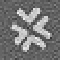
\includegraphics[height=\heightof{M}]{autanet.pdf}}
\definecolor{mygray}{gray}{0.333}
\iftypodisclaim%
\ifafour\newcommand\addprintnote{\begin{picture}(0,0)%
\put(245,149){\makebox(0,0){\rotatebox{90}{\tiny\color{mygray}\textsf{This
            document is designed for screen reading and
            two-up printing on A4 or Letter paper}}}}%
\end{picture}}% A4
\else\newcommand\addprintnote{\begin{picture}(0,0)%
\put(176,112){\makebox(0,0){\rotatebox{90}{\tiny\color{mygray}\textsf{This
            document is designed for screen reading and
            two-up printing on A4 or Letter paper}}}}%
\end{picture}}\fi%afourtrue
\makeoddfoot{plain}{}{\makebox[0pt]{\thepage}\addprintnote}{}
\else
\makeoddfoot{plain}{}{\makebox[0pt]{\thepage}}{}
\fi%typodisclaimtrue
\makeoddhead{plain}{\scriptsize\reporthead}{}{}
% \copypagestyle{manainitial}{plain}
% \makeheadrule{manainitial}{\headwidth}{0.5\normalrulethickness}
% \makeoddhead{manainitial}{%
% \footnotesize\sffamily%
% \scshape\headauthor}{}{\footnotesize\sffamily%
% \headtitle}
% \makeoddfoot{manaart}{}{\thepage}{}

\pagestyle{manaart}

\setlength{\droptitle}{-3.9\onelineskip}
\pretitle{\begin{center}\LARGE\sffamily%
\bfseries}
\posttitle{\bigskip\end{center}}

\makeatletter\newcommand*{\atf}{
\includegraphics[%trim=1pt 1pt 0pt 0pt,
totalheight=\heightof{@}]{atblack.png}}\makeatother
\providecommand{\affiliation}[1]{\textsl{\textsf{\footnotesize #1}}}
\providecommand{\epost}[1]{\texttt{\footnotesize\textless#1\textgreater}}
\providecommand{\email}[2]{\href{mailto:#1ZZ@#2 ((remove ZZ))}{#1\protect\atf#2}}

\preauthor{\vspace{-0.5\baselineskip}\begin{center}
\normalsize\sffamily%
\lineskip  0.5em}
\postauthor{\par\end{center}}
\predate{\DTMsetdatestyle{mydate}\begin{center}\footnotesize}
\postdate{\end{center}\vspace{-\medskipamount}}

\setfloatadjustment{figure}{\footnotesize}
\captiondelim{\quad}
\captionnamefont{\footnotesize\sffamily%
}
\captiontitlefont{\footnotesize}
%\firmlists
\midsloppy
% handling orphan/widow lines, memman.pdf
% \clubpenalty=10000
% \widowpenalty=10000
% \raggedbottom
% Downes, memman.pdf
\clubpenalty=9996
\widowpenalty=9999
\brokenpenalty=4991
\predisplaypenalty=10000
\postdisplaypenalty=1549
\displaywidowpenalty=1602
\raggedbottom

\paragraphfootnotes
% \threecolumnfootnotes
%\setlength{\footmarkwidth}{0em}
%\setlength{\footmarksep}{0em}
\footmarkstyle{\textsuperscript{%\color{myred}
\scriptsize\bfseries#1}~}
%\footmarkstyle{\textsuperscript{\color{myred}\bfseries#1}~}
%\footmarkstyle{\textsuperscript{[#1]}~}

\selectlanguage{british}\frenchspacing

%%%%%%%%%%%%%%%%%%%%%%%%%%%%%%%%%%%%%%%%%%%%%%%%%%%%%%%%%%%%%%%%%%%%%%%%%%%%
%%% Paper's details
%%%%%%%%%%%%%%%%%%%%%%%%%%%%%%%%%%%%%%%%%%%%%%%%%%%%%%%%%%%%%%%%%%%%%%%%%%%%
\title{\propertitle}
\author{%
\hspace*{\stretch{1}}%
%% uncomment if additional authors present
\parbox{0.49\linewidth}%\makebox[0pt][c]%
{\protect\centering P.G.L.  Porta Mana\\%
\footnotesize\epost{\email{piero.mana}{ntnu.no}}}%
\hspace*{\stretch{1}}%
\parbox{0.49\linewidth}%\makebox[0pt][c]%
{\protect\centering B. Jacobsen\\%
\footnotesize\epost{\email{bente.jacobsen}{ntnu.no}}}%
\hspace*{\stretch{1}}%
%\quad\href{https://orcid.org/0000-0002-6070-0784}{\protect\includegraphics[scale=0.16]{orcid_32x32.png}\textsc{orcid}:0000-0002-6070-0784}%
}

%\date{Draft of \today\ (first drafted \firstdraft)}
\date{\firstpublished; updated \updated}

%%%%%%%%%%%%%%%%%%%%%%%%%%%%%%%%%%%%%%%%%%%%%%%%%%%%%%%%%%%%%%%%%%%%%%%%%%%%
%%% Macros @@@
%%%%%%%%%%%%%%%%%%%%%%%%%%%%%%%%%%%%%%%%%%%%%%%%%%%%%%%%%%%%%%%%%%%%%%%%%%%%

% Common ones - uncomment as needed
%\providecommand{\nequiv}{\not\equiv}
%\providecommand{\coloneqq}{\mathrel{\mathop:}=}
%\providecommand{\eqqcolon}{=\mathrel{\mathop:}}
%\providecommand{\varprod}{\prod}
\newcommand*{\de}{\partialup}%partial diff
\newcommand*{\pu}{\piup}%constant pi
\newcommand*{\delt}{\deltaup}%Kronecker, Dirac
%\newcommand*{\eps}{\varepsilonup}%Levi-Civita, Heaviside
%\newcommand*{\riem}{\zetaup}%Riemann zeta
%\providecommand{\degree}{\textdegree}% degree
%\newcommand*{\celsius}{\textcelsius}% degree Celsius
%\newcommand*{\micro}{\textmu}% degree Celsius
\newcommand*{\I}{\mathrm{i}}%imaginary unit
\newcommand*{\e}{\mathrm{e}}%Neper
\newcommand*{\di}{\mathrm{d}}%differential
%\newcommand*{\Di}{\mathrm{D}}%capital differential
%\newcommand*{\planckc}{\hslash}
%\newcommand*{\avogn}{N_{\textrm{A}}}
%\newcommand*{\NN}{\bm{\mathrm{N}}}
%\newcommand*{\ZZ}{\bm{\mathrm{Z}}}
%\newcommand*{\QQ}{\bm{\mathrm{Q}}}
\newcommand*{\RR}{\bm{\mathrm{R}}}
%\newcommand*{\CC}{\bm{\mathrm{C}}}
%\newcommand*{\nabl}{\bm{\nabla}}%nabla
%\DeclareMathOperator{\lb}{lb}%base 2 log
%\DeclareMathOperator{\tr}{tr}%trace
%\DeclareMathOperator{\card}{card}%cardinality
%\DeclareMathOperator{\im}{Im}%im part
%\DeclareMathOperator{\re}{Re}%re part
%\DeclareMathOperator{\sgn}{sgn}%signum
%\DeclareMathOperator{\ent}{ent}%integer less or equal to
%\DeclareMathOperator{\Ord}{O}%same order as
%\DeclareMathOperator{\ord}{o}%lower order than
%\newcommand*{\incr}{\triangle}%finite increment
\newcommand*{\defd}{\coloneqq}
\newcommand*{\defs}{\eqqcolon}
\newcommand*{\Land}{\bigwedge}
\newcommand*{\Lor}{\bigvee}
%\newcommand*{\lland}{\DOTSB\;\land\;}
%\newcommand*{\llor}{\DOTSB\;\lor\;}
%\newcommand*{\limplies}{\mathbin{\Rightarrow}}%implies
%\newcommand*{\suchthat}{\mid}%{\mathpunct{|}}%such that (eg in sets)
%\newcommand*{\with}{\colon}%with (list of indices)
%\newcommand*{\mul}{\times}%multiplication
%\newcommand*{\inn}{\cdot}%inner product
%\newcommand*{\dotv}{\mathord{\,\cdot\,}}%variable place
%\newcommand*{\comp}{\circ}%composition of functions
%\newcommand*{\con}{\mathbin{:}}%scal prod of tensors
%\newcommand*{\equi}{\sim}%equivalent to 
\renewcommand*{\asymp}{\simeq}%equivalent to 
%\newcommand*{\corr}{\mathrel{\hat{=}}}%corresponds to
%\providecommand{\varparallel}{\ensuremath{\mathbin{/\mkern-7mu/}}}%parallel (tentative symbol)
\renewcommand*{\le}{\leqslant}%less or equal
\renewcommand*{\ge}{\geqslant}%greater or equal
\DeclarePairedDelimiter\clcl{[}{]}
%\DeclarePairedDelimiter\clop{[}{[}
%\DeclarePairedDelimiter\opcl{]}{]}
%\DeclarePairedDelimiter\opop{]}{[}
\DeclarePairedDelimiter\abs{\lvert}{\rvert}
%\DeclarePairedDelimiter\norm{\lVert}{\rVert}
\DeclarePairedDelimiter\set{\{}{\}}
%\DeclareMathOperator{\pr}{P}%probability
\newcommand*{\pf}{\mathrm{p}}%probability
\newcommand*{\p}{\mathrm{P}}%probability
%\newcommand*{\E}{\mathrm{E}}
%\renewcommand*{\|}{\nonscript\,\vert\nonscript\;\mathopen{}}
\renewcommand*{\|}[1][]{\nonscript\,#1\vert\nonscript\;\mathopen{}}
%\DeclarePairedDelimiterX{\cond}[2]{(}{)}{#1\nonscript\,\delimsize\vert\nonscript\;\mathopen{}#2}
%\DeclarePairedDelimiterX{\condt}[2]{[}{]}{#1\nonscript\,\delimsize\vert\nonscript\;\mathopen{}#2}
%\DeclarePairedDelimiterX{\conds}[2]{\{}{\}}{#1\nonscript\,\delimsize\vert\nonscript\;\mathopen{}#2}
%\newcommand*{\+}{\lor}
%\renewcommand{\*}{\land}
\newcommand*{\sect}{\S}% Sect.~
\newcommand*{\sects}{\S\S}% Sect.~
\newcommand*{\chap}{ch.}%
\newcommand*{\chaps}{chs}%
\newcommand*{\bref}{ref.}%
\newcommand*{\brefs}{refs}%
%\newcommand*{\fn}{fn}%
\newcommand*{\eqn}{eq.}%
\newcommand*{\eqns}{eqs}%
\newcommand*{\fig}{fig.}%
\newcommand*{\figs}{figs}%
\newcommand*{\vs}{{vs}}
%\newcommand*{\etc}{{etc.}}
%\newcommand*{\ie}{{i.e.}}
%\newcommand*{\ca}{{c.}}
%\newcommand*{\eg}{{e.g.}}
\newcommand*{\foll}{{ff.}}
%\newcommand*{\viz}{{viz}}
\newcommand*{\cf}{{cf.}}
%\newcommand*{\Cf}{{Cf.}}
%\newcommand*{\vd}{{v.}}
\newcommand*{\etal}{{et al.}}
%\newcommand*{\etsim}{{et sim.}}
%\newcommand*{\ibid}{{ibid.}}
%\newcommand*{\sic}{{sic}}
%\newcommand*{\id}{\mathte{I}}%id matrix
%\newcommand*{\nbd}{\nobreakdash}%
%\newcommand*{\bd}{\hspace{0pt}}%
%\def\hy{-\penalty0\hskip0pt\relax}
\newcommand*{\labelbis}[1]{\tag*{(\ref{#1})$_\text{r}$}}
%\newcommand*{\mathbox}[2][.8]{\parbox[t]{#1\columnwidth}{#2}}
%\newcommand*{\zerob}[1]{\makebox[0pt][l]{#1}}
\newcommand*{\tprod}{\mathop{\textstyle\prod}\nolimits}
\newcommand*{\tsum}{\mathop{\textstyle\sum}\nolimits}
%\newcommand*{\tint}{\begingroup\textstyle\int\endgroup\nolimits}
\newcommand*{\tland}{\mathop{\textstyle\bigwedge}\nolimits}
\newcommand*{\tlor}{\mathop{\textstyle\bigvee}\nolimits}
%\newcommand*{\sprod}{\mathop{\textstyle\prod}}
%\newcommand*{\ssum}{\mathop{\textstyle\sum}}
%\newcommand*{\sint}{\begingroup\textstyle\int\endgroup}
%\newcommand*{\sland}{\mathop{\textstyle\bigwedge}}
%\newcommand*{\slor}{\mathop{\textstyle\bigvee}}
%\newcommand*{\T}{^\intercal}%transpose
%%\newcommand*{\QEM}%{\textnormal{$\Box$}}%{\ding{167}}
%\newcommand*{\qem}{\leavevmode\unskip\penalty9999 \hbox{}\nobreak\hfill
%\quad\hbox{\QEM}}

%%%%%%%%%%%%%%%%%%%%%%%%%%%%%%%%%%%%%%%%%%%%%%%%%%%%%%%%%%%%%%%%%%%%%%%%%%%%
%%% Custom macros for this file @@@
%%%%%%%%%%%%%%%%%%%%%%%%%%%%%%%%%%%%%%%%%%%%%%%%%%%%%%%%%%%%%%%%%%%%%%%%%%%%
 \definecolor{notecolour}{RGB}{68,170,153}
\newcommand*{\puzzle}{{\fontencoding{U}\fontfamily{fontawesometwo}\selectfont\symbol{225}}}
%\newcommand*{\puzzle}{\maltese}
\newcommand{\mynote}[1]{ {\color{notecolour}\puzzle\ #1}}
\newcommand*{\widebar}[1]{{\mkern1.5mu\skew{2}\overline{\mkern-1.5mu#1\mkern-1.5mu}\mkern 1.5mu}}

% \newcommand{\explanation}[4][t]{%\setlength{\tabcolsep}{-1ex}
% %\smash{
% \begin{tabular}[#1]{c}#2\\[0.5\jot]\rule{1pt}{#3}\\#4\end{tabular}}%}
% \newcommand*{\ptext}[1]{\text{\small #1}}
%\DeclareMathOperator*{\argsup}{arg\,sup}
\newcommand*{\dob}{degree of belief}
\newcommand*{\dobs}{degrees of belief}
\newcommand*{\yI}{\varBeta}
\newcommand*{\yC}{C}
\newcommand*{\yc}{c}
\newcommand*{\statm}[1]{\textsl{\textsf{#1}}}
\newcommand*{\eq}{\mathrel{\!=\!}}
\newcommand*{\yf}{f}
\newcommand*{\yq}{q}
\newcommand*{\yth}{\theta}
\newcommand*{\ynu}{\bm{\nu}}
\newcommand*{\yN}{N}
\newcommand*{\yNa}{\widebar{N}}
\newcommand*{\yF}{\bm{F}}
\newcommand*{\yFm}[1][m]{\yF^{(#1)}}
\newcommand*{\yFFm}[1][m]{F^{(#1)}}
\newcommand*{\yh}{\bm{h}}
\newcommand*{\yhm}[1][m]{\yh^{(#1)}}
\newcommand*{\yH}{\bm{H}}
\newcommand*{\yHHm}[1][m]{H^{(#1)}}
\newcommand*{\yHm}[1][m]{\yH^{(#1)}}
\newcommand*{\yIm}[1][m]{I^{(#1)}}
\newcommand*{\yJm}[1][m]{T^{(#1)}}
\newcommand*{\yNm}[1][m]{N^{(#1)}}
\newcommand*{\yNma}[1][m]{\yNa^{(#1)}}
\newcommand*{\ycm}[1][m]{c^{(#1)}}
\newcommand*{\yFa}{\widebar{\yF}}
\newcommand*{\ySS}{S}
\newcommand*{\yS}{\bm{\ySS}}
\DeclarePairedDelimiter\tu{\{}{\}}
\newcommand*{\ymh}{\Hat{m}}
\newcommand*{\yih}{\Hat{\imath}}
\newcommand*{\yjh}{\Hat{t}}
\newcommand*{\yNhm}{\yNm[\ymh]}
\newcommand*{\yIhm}[1][m]{\Hat{I}^{(#1)}}
\newcommand*{\yJhm}[1][m]{\Hat{T}^{(#1)}}
\newcommand*{\yIh}{\Hat{I}}
\newcommand*{\yJh}{\Hat{T}}
\newcommand*{\ka}{\alpha}
\newcommand*{\kb}{\beta}
\newcommand*{\kam}[1][m]{\ka^{(#1)}}
\newcommand*{\kbm}[1][m]{\kb^{(#1)}}
%%% Custom macros end @@@

%%%%%%%%%%%%%%%%%%%%%%%%%%%%%%%%%%%%%%%%%%%%%%%%%%%%%%%%%%%%%%%%%%%%%%%%%%%%
%%% Beginning of document
%%%%%%%%%%%%%%%%%%%%%%%%%%%%%%%%%%%%%%%%%%%%%%%%%%%%%%%%%%%%%%%%%%%%%%%%%%%%
%\firmlists
\begin{document}
\captiondelim{\quad}\captionnamefont{\footnotesize}\captiontitlefont{\footnotesize}
\selectlanguage{british}\frenchspacing
\maketitle

%%%%%%%%%%%%%%%%%%%%%%%%%%%%%%%%%%%%%%%%%%%%%%%%%%%%%%%%%%%%%%%%%%%%%%%%%%%%
%%% Abstract
%%%%%%%%%%%%%%%%%%%%%%%%%%%%%%%%%%%%%%%%%%%%%%%%%%%%%%%%%%%%%%%%%%%%%%%%%%%%
\abstractrunin
\abslabeldelim{}
\renewcommand*{\abstractname}{}
\setlength{\absleftindent}{0pt}
\setlength{\absrightindent}{0pt}
\setlength{\abstitleskip}{-\absparindent}
\begin{abstract}\labelsep 0pt%
  \noindent Some memos on the problem of inferring connectivity by means of
  the probability-calculus aka Bayesian theory.
%\\\noindent\emph{\footnotesize Note: Dear Reader \amp\ Peer, this manuscript is being peer-reviewed by you. Thank you.}
% \par%\\[\jot]
% \noindent
% {\footnotesize PACS: ***}\qquad%
% {\footnotesize MSC: ***}%
%\qquad{\footnotesize Keywords: ***}
\end{abstract}
\selectlanguage{british}\frenchspacing

%%%%%%%%%%%%%%%%%%%%%%%%%%%%%%%%%%%%%%%%%%%%%%%%%%%%%%%%%%%%%%%%%%%%%%%%%%%%
%%% Epigraph
%%%%%%%%%%%%%%%%%%%%%%%%%%%%%%%%%%%%%%%%%%%%%%%%%%%%%%%%%%%%%%%%%%%%%%%%%%%%
% \asudedication{\small ***}
% \vspace{\bigskipamount}
% \setlength{\epigraphwidth}{.7\columnwidth}
% %\epigraphposition{flushright}
% \epigraphtextposition{flushright}
% %\epigraphsourceposition{flushright}
% \epigraphfontsize{\footnotesize}
% \setlength{\epigraphrule}{0pt}
% %\setlength{\beforeepigraphskip}{0pt}
% %\setlength{\afterepigraphskip}{0pt}
% \epigraph{\emph{text}}{source}



%%%%%%%%%%%%%%%%%%%%%%%%%%%%%%%%%%%%%%%%%%%%%%%%%%%%%%%%%%%%%%%%%%%%%%%%%%%%
%%% BEGINNING OF MAIN TEXT
%%%%%%%%%%%%%%%%%%%%%%%%%%%%%%%%%%%%%%%%%%%%%%%%%%%%%%%%%%%%%%%%%%%%%%%%%%%%

\section{Introduction}
\label{sec:intro}

We are interested in quantifying the proportion with which several brain
regions project to others. It's impossible, at least at present, to simply
count individual projections. What's done experimentally, with very clever
techniques, is analogous to survey sampling: we manage to see, more or less
clearly, a small sample of projections. From this sample we want to infer
the larger picture, for a single brain and on average for a
\enquote{typical} brain. We show here how to make such inferences using the
probability-calculus
\citep{jaynes1994_r2003,hailperin1996,soxetal1988_r2013}, also known as
Bayesian theory.

We accompany the method with an extensive discussion of its steps and
assumptions, for the sake of researchers unfamiliar with it. But we believe
that some of the points of view will be of interest also to experts in the
method.


\section{Synopsis of the problem}
\label{sec:synopsis}

We're considering two sets of neurons, which we call \emph{target} set and
\emph{input} set. The neurons in the target set are of several classes, for
example parvalbumin or somatostatin interneurons; and are distributed
across several regions, for example medial septal complex or thalamus).
Same holds for the input set. In general we are interested in the number of
projections of input neurons to target neurons, and in how such projections
are distributed across regions, or classes, or both, of neurons. More
specifically we focus here on the following kind of question: How many
input neurons in a region $R$ (independently of their class) project to
target neurons of class $C$ (in a specific location)? And we want to
compare the answer for several combinations of input regions $R$ and target
classes $C$, thus obtaining the proportion for each combination.

But the question above is still imprecise. Are we asking about a specific
mouse? or about the average across all mice having some specific
characteristics? These two cases can have slightly different answers, and
their difference is important for the application of the
probability-calculus and for experimental verification. We'll focus on
these two kinds of question:
\begin{description}[font=\itshape\mdseries]
\item[Individual:]\label{item:Qindiv} If we were able to perfectly count,
  in the next mouse to be examined, the number of input neurons in region
  $R$ projecting on average to a target neuron of class $C$, -- what number
  would we find?
\item[Collective or average:]\label{item:Qcollect} If we were able to
  perfectly count, for each mouse (with some specific traits such as age or
  gender and so on) to be examined in the future or that could have been
  examined in the past, the number of input neurons in region $R$
  projecting to target neurons of class $C$, -- what average number would
  we find?
\end{description}
It's intuitively clear that the answer to the second question comes from
the combination of answers to the first, for many mice. In either case, our
questions are about \emph{statistics}: total numbers, averages, deviations
from averages, and so on. 

\medskip

\textbf{The observations and data we use}: In a mouse, virus methodologies
allow us to select several neurons in the target set and to collectively
observe which neurons in the input set project to them. We can't
distinguish, however, which input neuron projects to which target neuron.
Such observations are made in several mice.

There's a complication: to make this kind of observation the mouse must be
killed. If it's killed too early, the virus hasn't had the time to spread
to all input neurons. If the mouse is killed too late, the starter neurons
decay and are no longer visible. So we also need to guess, for each
observed mouse, whether there were additional starter neurons, no longer
visible, and what proportion of input neurons have been reached by the
virus. As data we have the number of days between virus injection and
killing, for each mouse. This complication for the moment is set aside to
simplify the method, but will be taken into account later.

\medskip

Now let's sketch a schematic picture of the strategy to answer the two
questions above.

\section{Formulation and strategies}
\label{sec:strategies}

\setcounter{subsection}{-1}
\subsection{Preliminary remarks}
\label{sec:prelim_remarks}

Probabilistic inferences are just generalizations of logical inferences.
Their analysis therefore involve a logical analysis of the problem. A
probabilistic inference generally boils down to these steps:
\begin{enumerate}[label=\arabic*.]
\item \label{item:step_statements} Find a set of simple, factual
  statements, in terms of which the questions and the data can be
  formulated. These are called \enquote{atomic statements}; atomic in the
  sense that we won't analyse them into more precise statements. The choice
  of atomic statements is not unique and is mostly dictated by convenience.

\item \label{item:step_formulate_question_data} Express the data and the
  possible answers to the questions in terms of the atomic statements:
  \begin{equation}
    \label{eq:data_answ_as_combos}
    \begin{gathered}
      \text{\small data} = \textit{\small[some combination of atomic statements]},
      \\
      \text{\small answers} =
      \textit{\small[some combination of atomic statements]}.
    \end{gathered}
  \end{equation}
  
\item \label{item:step_joint_prob} Assign a joint probability distribution
  for all the possible combinations of these atomic statements,
  \begin{equation}
    \label{eq:p_atomic_stats_eg}
    \pf(\textit{\small[combination of atomic statements]} \| \yI).
  \end{equation}
  This probability distribution is called the \enquote{pre-data} or
  \enquote{prior} distribution, because it depends on our background
  information and assumptions, denoted by $\yI$, but not yet on the
  experimental data.


\item \label{item:step_calculate_probabilities} Use the
  probability-calculus to determine, from the pre-data
  distribution~\eqref{eq:p_atomic_stats_eg} and the
  expressions~\eqref{eq:data_answ_as_combos}, the probability for each
  answer of interest, conditional on the data observed and on the pre-data
  information:
  \begin{equation}
    \label{eq:basic_conditional_prob}
    \pf(\text{\small answer} \| \text{\small data}, \yI)
    =
    \frac{\pf(\text{\small answer}, \text{\small data} \| \yI)}
    {\pf(\text{\small data} \| \yI)}.
  \end{equation}
  The probabilities for all possible answers form the so-called
  \enquote{post-data} or \enquote{posterior} distribution.
\end{enumerate}

\begin{innote}
  Why do we need a pre-data distribution? can't we find the final
  probability from the data alone, without background information and
  assumptions? -- No, we can't; it's a logical impossibility. Just as in
  the truth-calculus (formal logic) we can't prove any theorem if we don't
  specify some initial axioms or postulates \citep[\sect~2.1
  p.~43]{barwiseetal1990_r2003}, so in the probability-calculus we can't
  derive any probabilities without some initial \enquote{probabilistic
    postulates} \citep{hailperin2011}[p.~182]{johnson1924}. \emph{All}
  statistical and probabilistic methods use assumptions.
\end{innote}

These steps are very interdependent and usually not faced sequentially. A
choice of atomic statements, for example, may lead to difficulties in the
assignment of the pre-data probabilities. Trying to simplify the latter
probabilities may lead us back to consider an alternative choice of atomic
statements.

The first and third steps always involve some degree of simplification and
abstraction of our problem, necessary for eliminating features of the
problem that are unimportant, and for making the problem mathematically and
computationally tractable. The third step often involves some mathematical
approximations.


\medskip

We now discuss these steps for our problem.


\subsection{Step 1: atomic statements}
\label{sec:step_statements}

In our case there are several possibilities for this first step, the choice
of atomic statements. Our choice below tries to simplify the problem, to
make it computationally tractable, without making it unrealistic.

We consider a very large number of mice: those we have observed and all
those that we might observe in the future or we could have observed in the
past. For our inferences to be valid, these mice must be judged
\enquote{similar} in some respects. We label each mouse with an index
$m=1,2,\dotsc$.

For the moment \emph{let's fix a specific input region}, for example the
medial septal complex or thalamus, \emph{and a specific target class}, for
example parvalbumin interneurons, in a specific target region. We'll
discuss later how to combine inferences about several input regions and target
classes.

For each mouse, we consider all neurons constituting the chosen input
region, labelling them $i=1,2,\dotsc, \yIm$, and all neurons constituting
the target class, labelling them $t=1,2,\dotsc, \yJm$. The total numbers
of these neurons can be different from mouse to mouse, hence the 
\enquote{$(m)$} subscript, which we shall use also for other quantities
that may vary from mouse to mouse.

The values of the three labels $i,t,m$ may be arbitrary or carry some
information. For example, $m$ may reflect a temporal order, and $i$, $t$
may each reflect a topographical order, for example ventral to dorsal. In
the next step, however, we'll assume such order to be unimportant.

\medskip


Now that we've labelled the mice and the input and target neurons of
interest, let's consider some simple, specific statements about
projections. for example:
\[\parbox{0.95\linewidth}{\statm{In mouse $m=3$, the neuron $i=5$ in the input
      region projects to the neuron $t=4$ of the target class.}}\]
Such a statement must be either true or false, even if we may not have the
experimental technology to look and see. If we could experimentally
ascertain each of these statements, for all mice $m$, input neurons $i$,
target neurons $t$, then our problem would be solved. We'd just have to
count, and we could report the exact projection proportions for each mouse,
and also averages across all mice. \emph{We'll use this kind of statements as our
atomic statements.}

The situation collectively described by these statements is visualized in
\fig~\ref{fig:cmij}. We plot a grid for each mouse $m$. Each row $i$ in the
grid represents a neuron in the input region, each column $t$ a neuron of
the target class. If in mouse $m$ neuron $i$ projects to neuron $t$, then
we colour the corresponding entry $(i,t)$ in grid $m$ in black; or we can
write down the number 1 in it. If it doesn't project, then we use white or
the number 0.
%%\setlength{\intextsep}{0.5ex}% with wrapfigure
\begin{figure}[t!]%{r}{0.4\linewidth} % with wrapfigure
 \centering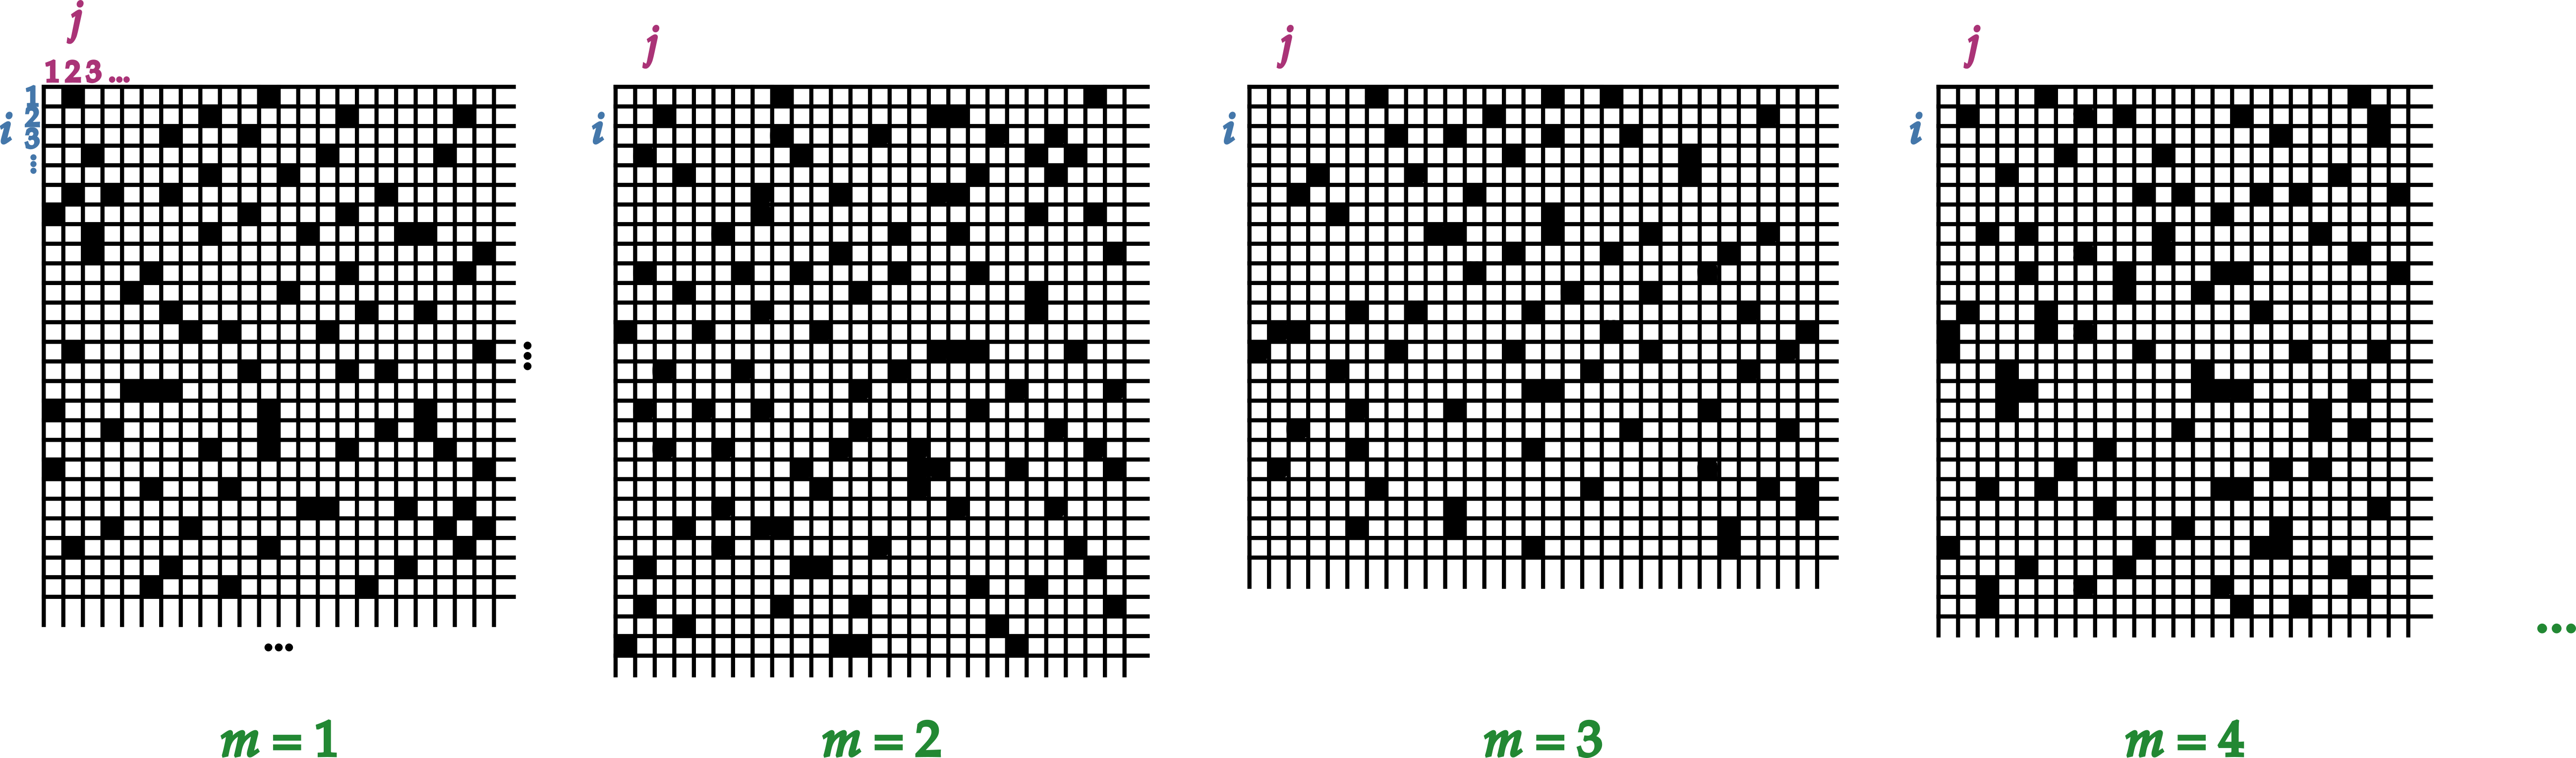
\includegraphics[width=\linewidth]{bente_notes_drawings.png}\\
 \caption{Imaginary layout of the connectivity from input to target region
   for all mice}\label{fig:cmij}
\end{figure}% bente_notes_drawings.svg

Let's indicate the entries of all grids with the binary indicators
$\ycm_{i t}$. If input neuron $i$ projects to target neuron $t$ in mouse
$m$, we write $\ycm_{i t}=1$; otherwise we write $\ycm_{i t}=0$. Then
\emph{our atomic statements will be of the form \enquote{$\ycm_{i t}=0$} or
  \enquote{$\ycm_{i t}=1$}} for all $m,i,t$ we need.

By assigning  a probability distribution for all combinations of these indicators,
\begin{equation}
  \label{eq:guess_prob_c}
  \pf(\tu{\ycm_{i t}} \| \yI)
  \equiv
  \pf\bigl(
  \ycm[1]_{1\,1}, \ycm[1]_{1\,2}, \dotsc,
  \ycm[1]_{2\,1}, \ycm[1]_{2\,2}, \dotsc,\;
  \ycm[2]_{1\,1}, \dotsc
  \|  \yI\bigr),
\end{equation}
we can calculate from it the
probabilities~\eqref{eq:basic_conditional_prob} for the answers to our main
questions.

First let's see how to express those answers and our data in terms of the
atomic statements.

\subsection{Step 2: data and answers in terms of atomic statements}
\label{sec:data_as_atomic}

\subsubsection{Our questions}
\label{sec:atomic_questions}

Let's start with the answers to our questions. As discussed in
\sect~\ref{sec:synopsis}, our questions are about individual and collective
statistics. Let's then introduce some statistics, expressed in terms of the
atomic statements.

Consider first a specific mouse $m$ and target neuron $t$. A useful
statistics is the total number of input neurons that project to that target
neuron. Denote this by $\yNm_{t}$. It is of course given by
\begin{equation}
  \label{eq:def_Nj}
  \yNm_{t} \defd \sum_{i} \ycm_{i t},
\end{equation}
that is, by counting the black squares in the $t$th column of the $m$th
grid in \fig~\ref{fig:cmij}.

This statistic is useful because from it we can calculate, for example, the average
number of projections to the target neurons in that mouse:
\begin{equation}
\yNma \defd \frac{1}{\yJm}\sum_{t}\yNm_{t},\label{eq:aver_proj_m}
\end{equation}
and the variance from that average,
\begin{equation}
\frac{1}{\yJm}\sum_{t}\bigl(\yNm_{t}-\yNma\bigr)^{2},\label{eq:variance_proj_m}
\end{equation}
which answer some basic questions about a specific mouse.

But we may be interested in a more statistics of the projections in that
mouse. For example, how many target neurons receive no projections from the
input region? how many receive only one projection? how many receive two?
And so on. This statistics is given by a histogram
$\yHm\defd \bigl(\yHHm_{0},\yHHm_{1}, \yHHm_{2},\dotsc, \yHHm_{\yIm}\bigr)$
of the number of projections for that mouse: $\yHHm_{0}$ is the number of
neurons receiving no projections, $\yHHm_{1}$ the number receiving only one
projection, and so on, up to the total number of neurons $\yIm$ in the
input region. Mathematically this histogram is given by
\begin{equation}
   \label{eq:count_histogram}
    \yHHm_{n} \defd \tsum_{t} \delt\bigl(\yNm_{t} = n\bigr)
\end{equation}
where $\delt$ is the Kronecker delta. From such histogram we can calculate
the mean and variance above; for example
$\yNma = \frac{1}{\yIm}\sum_{n}n\,\yHHm_{n}$.

Also useful is the normalized version of the histogram,
$\yFm \defd \yHm/\yJm$, corresponding to the relative frequency
distribution of projections.

\medskip

At the level of the whole mouse population (or subpopulation with specific
traits, as discussed before), we are interested again on the average number
of projections from the input region to an target neuron, and so on. But we
can ask for more statistical information. For example, if we had the
histograms $\yFm$ for each mouse $m$, we could then ask about the average
histogram of projections $\yFa \defd \frac{1}{M}\sum_{m} \yFm$ across the
whole population, where $M$ is the total number of mice. We could also ask
about the variance from such an average histogram. More in detail, we could
build a \enquote{super-statistics} or \enquote{histogram of histograms}: we
imagine to check every mouse, and for each we write down its histogram of
projections $\yFm$; then we count how many mice have the particular
histogram $\yF'$ in common, how many have another particular histogram
$\yF''$ in common, and so on. We obtain a \enquote{super-histogram}
$\yS=(\ySS_{\yF})$: $\ySS_{\yF'}$ is the proportion of mice that have the
same histogram $\yF'$, and so on. Mathematically it's expressed as
  \begin{equation}
    \label{eq:count_superhistogram}
    \ySS_{\bm{f}} \defd \frac{1}{M} \tsum_{m} \delt\bigl(\yFm = \bm{f}\bigr),
\end{equation}
similarly to the expression for the individual
statistics~\eqref{eq:count_histogram}. It allows us to say what's the most
common histogram of projections in our mice population, what's the average
histogram, and how much the histograms can vary from the average one,
across the population. Since each possible $\yFm$ is a tuple with $\yIm+1$
elements, the distribution $\yS$ is over an $(I+1)$-dimensional space,
where $I$ is the largest of all $\yIm$.


\subsubsection{Our data}
\label{sec:atomic_data}


The expression of the data in terms of the atomic statements
$\tu{\ycm_{i t}}$ requires some more thinking. We're still focusing on a
specific input region (say, thalamus) and a specific target class (say,
parvalbumin). Our data consists, for a number of mice, of the total number
of target neurons marked by the virus, and the total number of input
neurons that have been infected by the target ones, and thus also marked by
the virus. Let's use a circumflex to indicate observed quantities. The
observed mice are indexed with $\ymh$, the marked target neurons with
$\yjh$, and the marked input neurons with $\yih$. The total numbers of
marked target and input neurons in mouse $\ymh$ are $\yJhm$ and $\yIhm$.

Consider a specific mouse (we omit its index $\ymh$ for the moment), and
the grid that represents its projections. Owing to our assumption that the
specific order and indexing of target and input neurons doesn't matter, we
can rearrange the grid so that the input neurons marked by the virus are
the first $\yIh$ rows, and the marked target neurons are the first $\yJh$
columns; see \fig~\ref{fig:datamouse}.

Because of the way the virus infection works, our data correspond to the
following two main pieces of information; refer to the grid of
\fig~\ref{fig:datamouse}:
\begin{itemize}
\item[\textcolor{myred}{$\ka$}:] Each marked input neuron must project to
  \emph{at least one} marked target neuron -- otherwise it wouldn't have
  been infected and marked. This means that \emph{each row} in the
  upper-right, \textcolor{myred}{red-bounded} part of the grid \emph{must
    have at least one black entry} -- but we don't know how many black
  entries and where.
\item[\textcolor{mypurpleblue}{$\kb$}:] The unmarked input neurons
  \emph{cannot} project to the marked target neurons -- because otherwise
  they would have been infected and would be marked instead. Thus the
  lower-right, \textcolor{mypurpleblue}{blue-bounded} part of the grid has
  no black entries.
\end{itemize}
%%\setlength{\intextsep}{0.5ex}% with wrapfigure
\begin{figure}[t!]%{r}{0.33\linewidth} % with wrapfigure
 \centering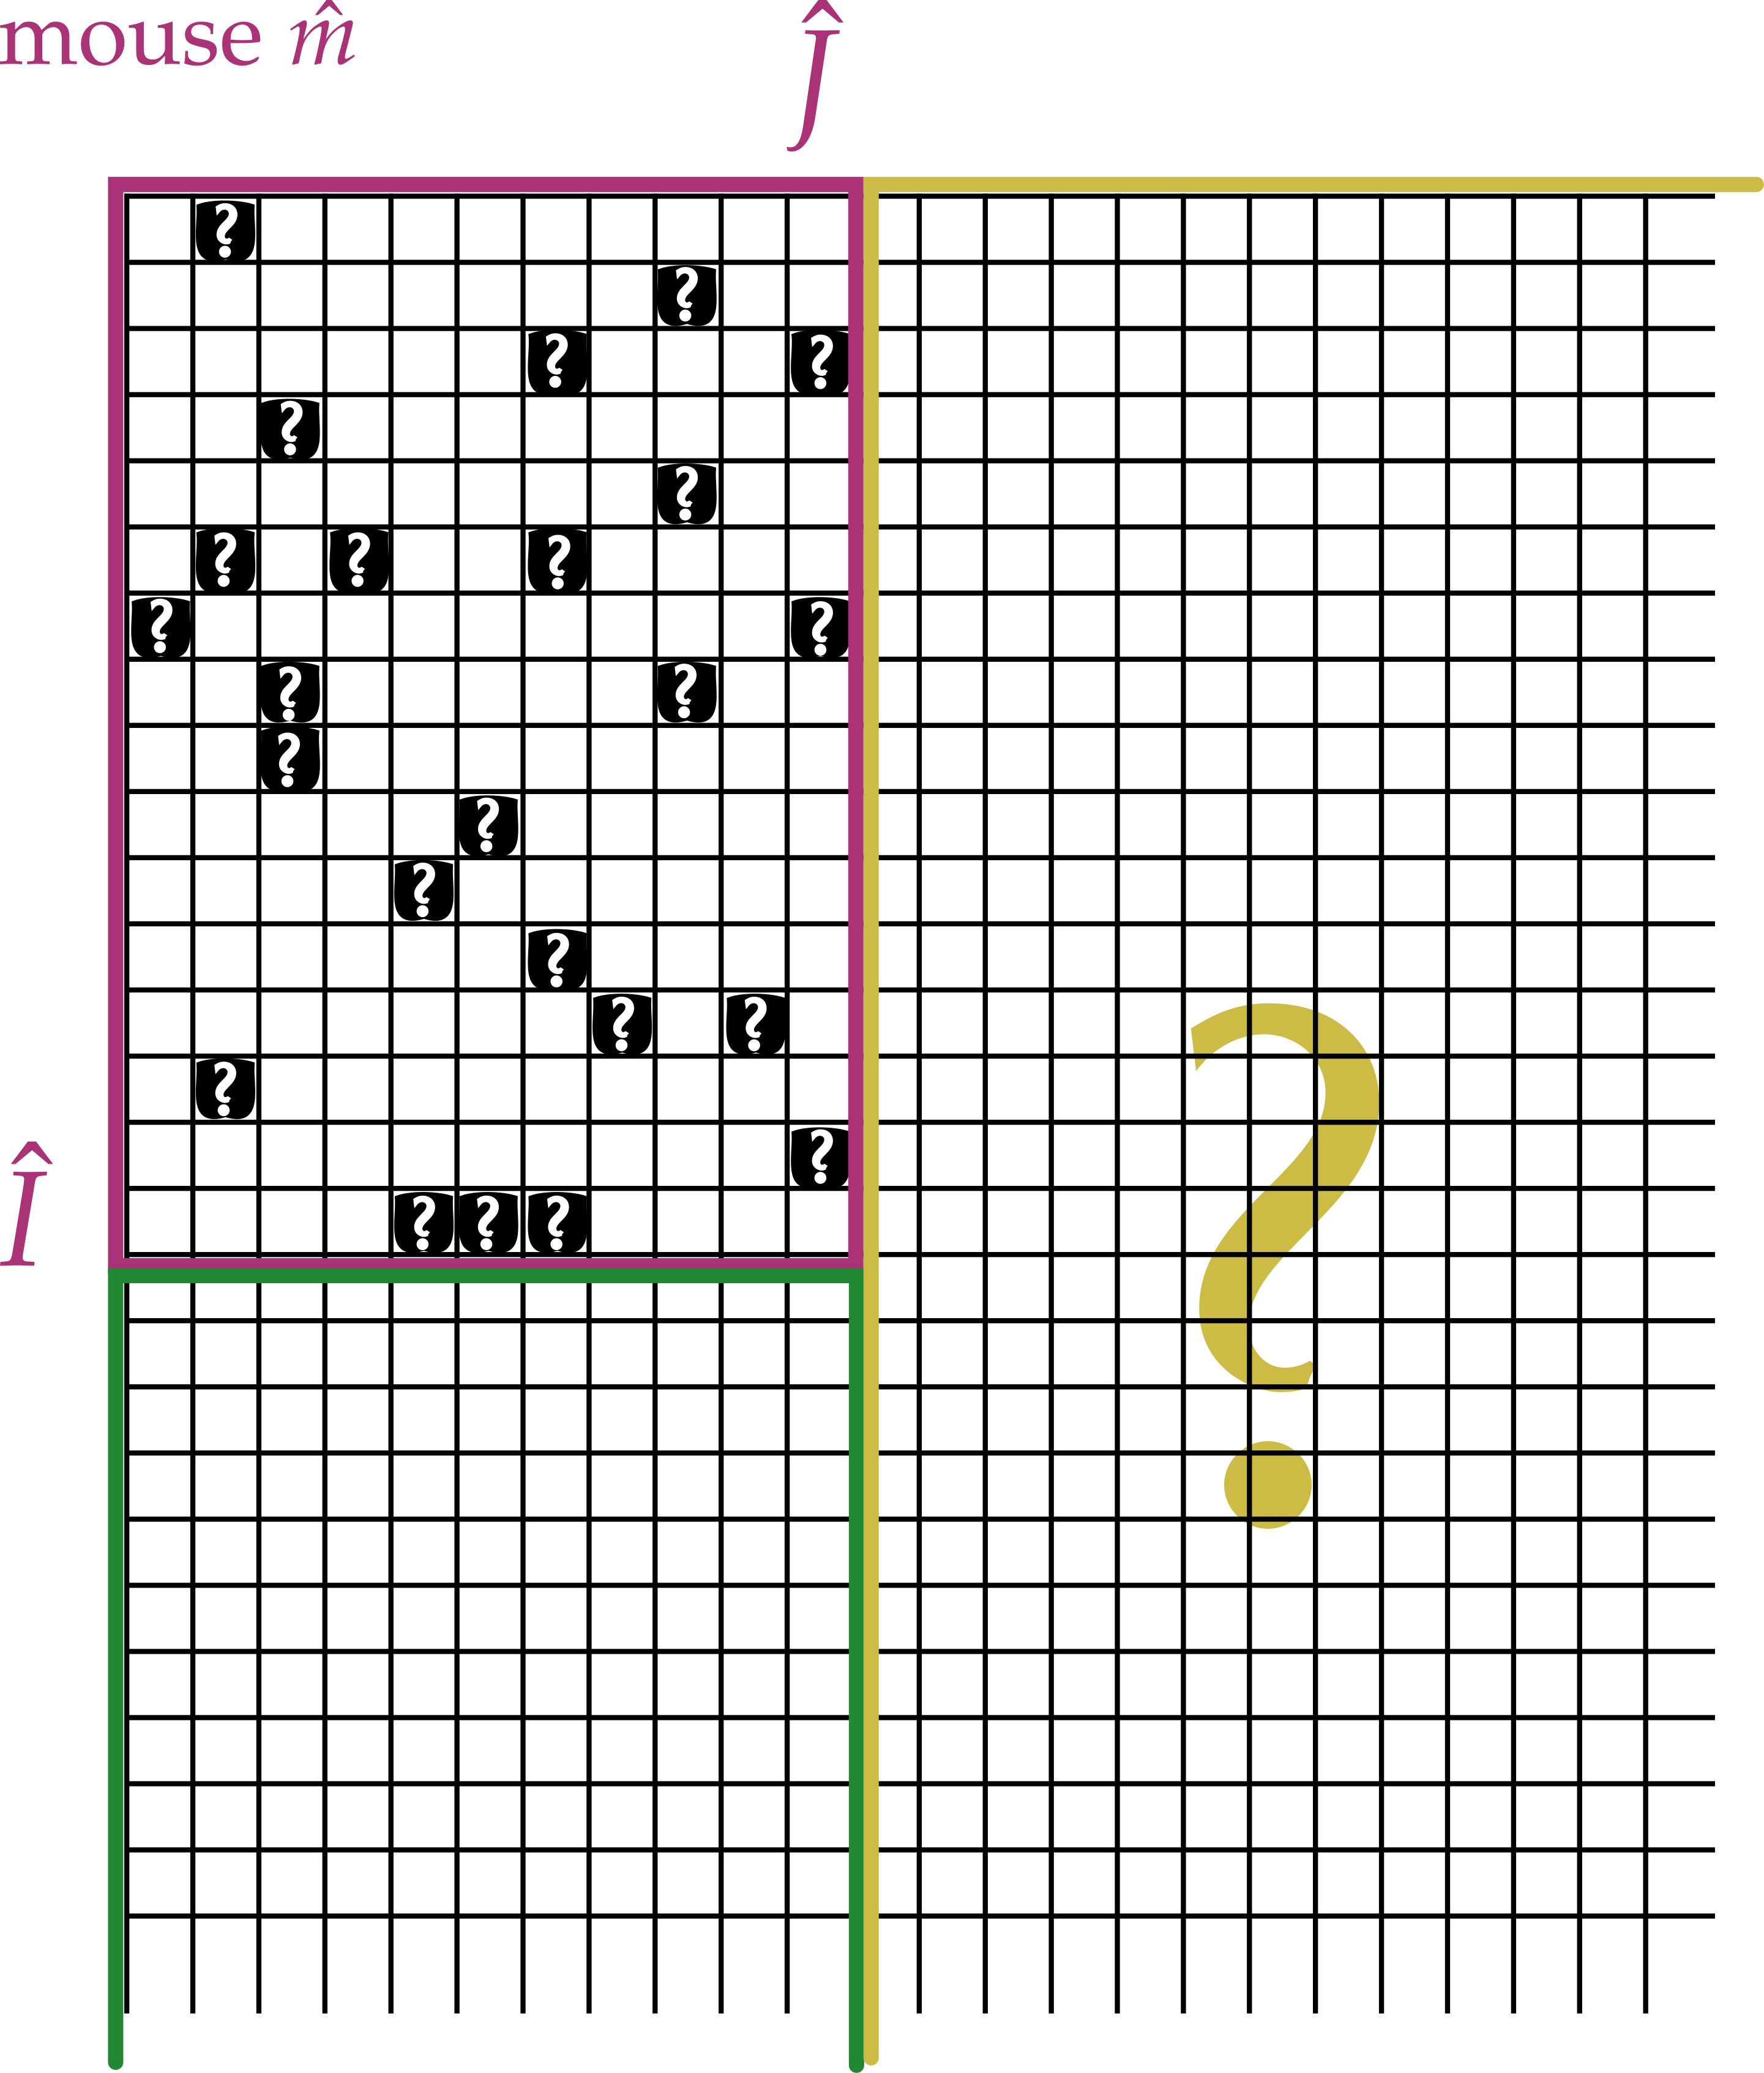
\includegraphics[width=0.5\linewidth]{data_mouse2.png}\\
 \caption{Imaginary layout of the connectivity data for an observed mouse}\label{fig:datamouse}
\end{figure}% data_mouse.svg
On the other hand we don't know anything about the projections of marked
and unmarked input neurons to the unmarked target neurons. This is
represented by the \textcolor{myyellow}{yellow-bounded} region on the right
with the large yellow question mark.

The expression of $\kb$ is simple: it corresponds to
\begin{equation}
  \label{eq:alpha_and}
\kb:\qquad  c_{i t} =0 \quad\text{for }i=\yIh+1,\dotsc, I
  \quad\text{and }t=1,\dotsc,\yJh.
\end{equation}

The expression of $\ka$ is slightly more involved. Fix a row $i$; the
statement that this row is empty is \enquote{$c_{i t}=0$ for
  $t=1, \dotsc, \yJh$}. Such a statement must be false (because a row must
contain at least one black entry), whether we choose the row $i=1$, or
$i=2$, and so on to $i=\yIh$. Then
\begin{equation}
  \label{eq:alpha_and}
  \begin{aligned}
  \ka:\qquad \text{not }\bigl[ &(c_{1 t} =0 \quad\text{for }t=1,\dotsc,\yJh)
\\  &\text{or }
  (c_{2 t} =0 \quad\text{for }t=1,\dotsc,\yJh)
    \\  &\text{or } \dotsb
    \\&\text{or }
  \bigl(c_{\yIh t} =0 \quad\text{for }t=1,\dotsc,\yJh \bigr)\bigr],
  \end{aligned}
\end{equation}
which can be more compactly written using Boolean logical operators as
\begin{equation}
  \label{eq:alpha_and_boole}
    \ka:\qquad \lnot \tlor_{i=1}^{\yIh} \bigl[
\tland_{t=1}^{\yJh} (c_{i t} \eq 0)
    \bigr].
\end{equation}

\medskip

The statements $\ka$ and $\kb$ above refer to a specific mouse $m$. To
express our data about all mice we simply \enquote{and} these statements
for all $m$.

Now that our data and the answers to our questions have been expressed as
combinations of atomic statements, we turn to the pre-data probability
distribution of the latter.


\subsection{Step 3: pre-data probabilities for the atomic statements}
\label{sec:step_joint_prob}

We must now assign the pre-data probabilities
\begin{equation}
  \labelbis{eq:guess_prob_c}
  \pf(\tu{\ycm_{i t}} \| \yI)
  % \equiv
  % \pf\bigl(
  % \ycm[1]_{1\,1}, \ycm[1]_{1\,2}, \dotsc,
  % \ycm[1]_{2\,1}, \ycm[1]_{2\,2}, \dotsc,\;
  % \ycm[2]_{1\,1}, \dotsc
  % \|  \yI\bigr),
\end{equation}
for all possible combinations of any number of atomic statements
$\ycm_{i t}$.


This probability distribution represents our pre-data guess about the
numbers presence or absence of projections. It should be a reasonable,
unbiased guess.
\begin{innote}
  Some researchers feel uncomfortable in quantifying such a guess. But, as
  we stressed in \sect~\ref{sec:strategies}, such a quantification is
  unavoidable: without it our experimental observations could not be
  probabilistically generalized to other neurons or mice. Some researchers
  also believe that there are statistical methods, such as so-called
  frequentist ones, which avoid this kind of pre-data assumptions. This is
  a mistaken belief. Those methods \emph{do} make pre-data assumptions, but
  misleadingly keep them hidden. % The advantage of the Bayesian approach is
  % that the pre-data assumptions are explicitly stated instead.
  As I. J. Good said: \enquote{The main difference is that in a
    non-Bayesian analysis more is swept under the carpet. This makes
    non-Bayesian methods politically expedient. The Bayesian is forced to
    put his cards on the table instead of up his sleeve. He thus helps
    others to improve his analysis, and this is always possible in a
    problem concerning the real world} \citep[\sect~2.3 p.~26]{good1969}
  (Good was Turing's collaborator in the breaking of the \emph{Enigma} code
  during World War II, using probabilistic methods). In fact, as the amount
  of experimental data increases, the effect of our pre-data guesses
  usually decreases. The Bayesian approach allows us to quantify this
  dependence and thus to decide whether the data we have collected are
  enough or whether we want to collect more.
\end{innote}


To assign this distribution we are going to use three \emph{symmetry}
assumptions, at three increasing levels of generality: about the statistics
$\yNm_{t}$ for each individual target neuron of each individual mouse;
about the statistics $\yFm$ for each individual mouse; and finally about
the super-statistics $\yS$ for all mice.


\subsubsection{$\ycm_{i t}$ for one target neuron and mouse:
  exchangeability}
\label{sec:oneneuron_exch}

Let's start by focusing on a specific but arbitrary target neuron in a
specific but arbitrary mouse $m$. We'll suppress all \enquote{$(m)$} for
the moment, to make the notation lighter.

Suppose we know the total number $N_{t}$ of projections to that neuron from
the input region, but not which neurons in the input neurons are
projecting. We want to assign the probability distribution for the
projection indicators $c_{1 t}$, $c_{2 j}$, and so on, conditional on
knowledge of $N_{t}$. Our assumption is this: \emph{there isn't any reason
  to believe that some input neuron $i'$ projects to $t$, more than some
  other input neuron $i''$}. In other words, the specific index $i$ of an
shouldn't give us any special information about the projection. This is
called an \emph{exchangeability} assumption.  In
which cases can this assumption be at least approximately justified?

One case is if the indexing of the input neurons is done in a way
completely unknown to us, for example by an automated unique-string
generator. This isn't our case, because no matter how an input neuron is
indexed we can always check what its location was. Another case is if all
input neurons under consideration are very similar, and very close with
respect to larger brain scales. Then none of them should find it easier to
project than any other. A third case is if previous studies showed that the
relative locations and morphological differences of the input neurons are
unimportant.

The exchangeability assumption may therefore be unreasonable if the input
neurons are located in widely different brain areas. In the latter case we
can sort them into small neighbourhood (and morphology) groups, and apply
the exchangeability assumption only within neighbourhoods. This is
equivalent to redefining the input region $R$ to a smaller one.

Exchangeability has a powerful mathematical consequence, called the
de~Finetti's representation theorem \citep{definetti1930,hewittetal1955}[a
more intuitive explanation is in][]{heathetal1976}[for an informative
review:][]{dawid2013}[the particular form used here is discussed
in][]{diaconis1977,diaconisetal1980}. Effectively it's a combinatorial
argument based on the assumed symmetry.

In our case, suppose we are interested in $n=n_{0}+n_{1}$ input neurons,
and we want the conditional probability that $n_{0}$ of them don't project
to $t$, so that their indicators $c_{i t}$ are $0$, and the other $n_{1}$
do project to $t$, and their indicators are $1$. We know that there are $I$
neurons in the whole input region, and that $N_{t}$ of these project. By
the assumed symmetry, this situation is equivalent to \enquote{drawing
  without replacement}, described by the hypergeometric distribution \citep[\chap~3]{jaynes1994_r2003}:
\begin{equation}
  \label{eq:hyperg_Nj}
  \pf(\tu{\underbracket{c_{\dotso t}=0}_{\mathclap{\text{$n_{0}$ of them}}}},
  \;\tu{\underbracket{c_{\dotso t}=1}_{\mathclap{\text{$n_{1}$ of them}}}} \| N_{t}, \yI)
  =
\frac{1}{\binom{n}{n_{0},n_{1}}}  \binom{N_{t}}{n_{1}}\binom{I-N_{t}}{n_{0}}\bigg/ \binom{I}{n},
\end{equation}
where the parentheses on the right are binomial coefficients. This
distribution simply comes from counting in how many ways we can draw
$n_{0}$ white and $n_{1}$ black balls from an urn containing $I-N_{t}$
white and $N_{t}$ black ones. The term $\binom{n}{n_{0},n_{1}}$ is a
multinomial coefficient, necessary because we are asking about the
probability of a specific set of input neurons.

We have such distribution separately for each target neuron $t$. But the
collection of these distributions depend on knowledge of all the
$\tu{N_{t}}$, which we don't know. We consider our guess about them next.



\subsubsection{$\yNm_{t}$ for one mouse}
\label{sec:onemouse_exch}

We're still focusing on a specific but arbitrary mouse $m$. Now we want to
express our guesses about the numbers of projections $N_{t}$ to a specific
set of $h$ target neurons.

Suppose we know the statistics $\yF=(F_{0}, F_{1}, \dotsc, F_{I})$,
described in \sect~\ref{sec:atomic_questions}, of such numbers of
projections for all $T$ target neurons. That is, $F_{0}$ is the proportion
of all target neurons receiving no projections from the input region,
$F_{1}$ the proportion receiving one projection, and so on. The number of
target neurons in each case is given by $T\,F_{n} \equiv H_{n}$.

We make again an assumption of symmetry: \emph{there isn't any reason for
  some target neuron $j'$ to have more or less projections than some other
  target neuron $j''$}. This is again an assumption of exchangeability, and
the discussion of its validity is analogous to that of the previous
section.

The result for our guesses is also similar. Our situation in this case is
analogous to \enquote{drawing without replacement} from an urn having $T$
balls of $I+1$ different colours or kinds (corresponding to the cases of
$0$ to $I$ projections), with proportions $(F_{0}, \dotsc, F_{I})$. We ask
in how many ways we can draw $h$ specific balls with proportions
$(f_{0}, \dotsc, f_{I})$, some of which may be zero. A counting argument
leads to the multivariate hypergeometric distribution
\citep[\chap~39]{johnsonetal1969_r1996}:
\begin{multline}
  \label{eq:definetti_Nj_finite}
  \pf(\tu{\underbracket{N_{\dotso}=0}_{\mathclap{\text{$hf_{0}$ of them}}}},
  \;\tu{\underbracket{N_{\dotso}=1}_{\mathclap{\text{$hf_{1}$ of them}}}},
\;\dotsc
  \;\tu{\underbracket{N_{\dotso}=I}_{\mathclap{\text{$hf_{I}$ of them}}}}
  \| \yF, \yI)
  ={}\\
  \frac{1}{\binom{h}{hf_{0},\dotsc,hf_{I}}}
  \binom{JF_{0}}{hf_{0}}\times\dotsm\times\binom{JF_{I}}{hf_{I}}\bigg/
  \binom{T}{h}.
\end{multline}

If our question is about a small set of $h$ neurons compared to the total
number $T$, and the proportions $f_{t}$ are small compared to $1$, the
formula above has a useful approximation:
\begin{equation}
  \label{eq:definetti_Nj_infinite_approx}
  \pf(\tu{\underbracket{N_{\dotso}=0}_{\mathclap{\text{$hf_{0}$ of them}}}},
  \;\tu{\underbracket{N_{\dotso}=1}_{\mathclap{\text{$hf_{1}$ of them}}}},
\;\dotsc
  \;\tu{\underbracket{N_{\dotso}=I}_{\mathclap{\text{$hf_{I}$ of them}}}}
  \| \yF, \yI)
\approx
% \int\!\!\!\di\yF\;
% \pf(\yF \| \yI)\;
% F_{N_{1}} \times \dotsm \times F_{N_{h}}
% \equiv{}\\[-2\jot]
% \int\!\!\!\di\yF\;
% \pf(\yF \| \yI)\; 
\prod_{n=0}^{I}(F_{n})^{hf_{n}}.
\end{equation}
The integral appears because we approximate the tuple $\yF$ as a continuous
quantity. It takes values in an $(I+1)$-dimensional space.

\medskip

We have one such distribution separately for each mouse. But the collection
of these distributions depend on the statistics $\tu{\yFm}$, which we don't
know. We discuss our guess about them next


\subsubsection{$\yFm$ for the mouse population}
\label{sec:allmice_exch}

So far we have expressed our guess about the projection indicators
$\tu{\ycm_{i t}}$ conditional on the number of projections $\tu{\yNm_{t}}$
and our guess about these numbers conditional on the statistics
$\tu{\yFm}$. Let's finally consider our guess about these statistics.

We proceed analogously as in the previous two guesses, by assuming that
we know the \enquote{super-statistics} $\yS$ about the statistics
$\tu{\yFm}$ of all mice. This time, however, we'll also assign a guess for
$\yS$ without relying on higher-level statistics. We also make an analogous
symmetry assumption, this time about the mouse population.

The result is analogous to the guess about $\tu{\yNm_{t}}$. This time we
use the analogous version of the approximate
form~\eqref{eq:definetti_Nj_infinite_approx}, since the number of mice is
in principle infinite, for the happiness of exterminator companies:
\begin{equation}
  \label{eq:distr_H_mice}
  \pf( \underbracket{\yFm[1], \yFm[2], \dotsc}_{\text{any number}} \| \yS, \yI) =
  % \int\!\!\!\di \yS\;
  % \pf(\yS \| \yI)\;
  \ySS_{\yFm[1]} \times \ySS_{\yFm[2]} \times \dotsm\;.
\end{equation}

The super-statistics $\yS$ is unknown to us. Our pre-data guess about it is
expressed by a probability density $\pf(\yS \| \yI)\,\di\yS$. It turns out
that the exact form of this density is unimportant if we have numerous
data, because the data will change its shape to reflect the observed
statistics. For the moment we assume it to be constant:
\begin{equation}
  \label{eq:distr_lambda}
  \pf(\yS \| \yI) = \text{const.}
\end{equation}
but later we'll check if changes in this distribution lead to important
changes in our final inferences.

\subsubsection{Final form for our pre-data distribution}
\label{sec:final_predata}

The final form of our pre-data distribution is obtained by combining the
distributions~\eqref{eq:hyperg_Nj} and \eqref{eq:definetti_Nj_finite} for
each mouse of interest, together with \eqref{eq:distr_H_mice} and
\eqref{eq:distr_lambda}. And summing over all possible values of $\yS$, of
all $\tu{\yFm}$ and of all $\tu{\yNm_{t}}$. We don't write this down,
because some of those sums won't be necessary when we calculate the
probability of the desired answers given our data.

\subsection{Step 4: the probability for the answers given the data}
\label{sec:step4_answer_from_data}

Our final goal is to guess the projection statistics $\yFm$ for the
experimentally observed mice $\tu{m}$, and the super-statistics $\yS$
for the whole mouse population under study, given our experimental data and
pre-data information:
\begin{equation}
  \label{eq:guess_given_data}
  \pf(\underbracket{\tu{\yFm}}_{\mathclap{\text{observed mice}}}, \yS
  \| \text{\small data}, \yI).
\end{equation}
This conditional probability can be calculated in different ways. The most
convenient for our problem is Bayes's theorem, because it relates this
conditional probability to one with data and statistics inverted:
\begin{equation}
  \label{eq:bayes_data_answers}
  \pf(\tu{\yFm}, \yS
  \| \text{\small data}, \yI)
  \propto
  \pf( \text{\small data} \|
  \tu{\yFm}, \yS, \yI)
  \times \pf( \tu{\yFm}, \yS \| \yI)
\end{equation}
The probability distribution on the right is useful because it has the
unknown statistics in the conditional, allowing us to use the pre-data
probabilities of \sect~\ref{sec:step_joint_prob}. The product on the right
can be found, apart from a normalizing constant, by sampling methods such
as Monte Carlo.


\medskip

We now find the probability of the data, assuming for the moment that all
statistics $\yS$, $\tu{\yFm}$, $\tu{\yNm_{t}}$ are known.

The data consist in the two main statements $\kam$ and $\kbm$, discussed in
\sect~\ref{sec:atomic_data}, for all observed mice $\tu{m}$. Let's first
focus on one specific mouse and omit \enquote{$(m)$}. We calculate the
probability for the data as follows:
\begin{multline}
  \label{eq:alph_beta_given_stats}
  \pf( \ka,\kb \|\tu{N_{t}},  \yF, \yS, \yI) ={}\\
  \pf( \ka \|\kb, \tu{N_{t}},  \yF, \yS, \yI) \times
    \pf( \kb \|\tu{N_{t}},  \yF, \yS, \yI).
\end{multline}

The last factor is easily calculated using formula~\eqref{eq:hyperg_Nj}
with $n_{0}=I-\yIh$ and $n_{1}=0$:
\begin{multline}
  \label{eq:kb_given_stats}
  \pf( \kb \|\tu{N_{t}},  \yF, \yS, \yI) \equiv
  \pf(\tu{\underbracket{c_{\dotso,1}=0}_{\mathclap{\text{$I-\yIh$ of them}}}},
  \dotsc,
  \tu{\underbracket{c_{\dotso,\yJh}=0}_{\mathclap{\text{$I-\yIh$ of them}}}}
  \|\tu{N_{t}},  \yF, \yS, \yI)
  ={}\\
  \prod_{t=1}^{\yJh}
  \binom{N_{t}}{0}\binom{I-N_{t}}{I-\yIh}
  \bigg/ \binom{I}{I-\yIh}
  \equiv
  \prod_{t=1}^{\yJh}
\binom{\yIh}{N_{t}}\bigg/ \binom{I}{N_{t}}.  
\end{multline}
This results makes sense: for each column $t$, the denominator
$\binom{I}{N_{t}}$ counts the total number of ways in which $N_{t}$ black
entries can be distributed among $\yIh$ places. The numerator
$\binom{\yIh}{N_{t}}$ counts the number of ways in which the $N_{t}$ black
entries can be limited to the first $\yIh$ places, leaving the remaining
$I-\yIh$ blank, as requested by our data $\kb$.


Now to $\pf( \ka \|\kb, \tu{N_{t}}, \yF, \yS, \yI)$. By the Boolean
expression of $\ka$, \eqn~\eqref{eq:alpha_and_boole},
\begin{multline}
  \label{eq:p_ka_boole}
  \pf( \ka \|\kb, \tu{N_{t}}, \yF, \yS, \yI) \equiv
  \pf\Bigl\{
\lnot \tlor_{i=1}^{\yIh} \bigl[
\tland_{t=1}^{\yJh} (c_{i t} \eq 0)
    \bigr]
    \|\dotso \Bigr\} ={}\\
    1-
  \pf\Bigl\{
\tlor_{i=1}^{\yIh} \bigl[
\tland_{t=1}^{\yJh} (c_{i t} \eq 0)
    \bigr]
    \|\dotso \Bigr\} ={}\\
    \begin{aligned}[b]
    1&-
\sum_{i=1}^{\yIh} \pf\bigl[
\tland_{t=1}^{\yJh} (c_{i t} \eq 0) \|\dotso \bigr]
\\&+
\sum_{i',i''}^{i'> i''} \pf\bigl[
\tland_{t=1}^{\yJh} (c_{i'\,t} \eq 0)\;
\tland_{t=1}^{\yJh} (c_{i''\,t} \eq 0)
\|\dotso \bigr]
\\&- \dotsb\text{ \small[terms with three and more $i$]}.
    \end{aligned}
\end{multline}
Where we have indicated the conditional with $\dotso$ for brevity. For the
first equality we have used the rule for probability of the negation of a
statement. For the second equality we have used the sum rule of probability
for \emph{non}-mutually exclusive statements. In fact, the expression
$\tland_{t=1}^{\yJh} (c_{i t} \eq 0)$ says that the $i$th row is empty, but
this doesn't exclude that other rows be empty as well.

Each summand in the last expression is calculated using
formula~\eqref{eq:hyperg_Nj}. Consider the generic term with $r$ different $i$s:
\begin{multline}
  \label{eq:generic_term_disjunction_p}
(-1)^{r}  \pf\bigl[
\underbracket{\tland_{t=1}^{\yJh} (c_{\dotso\,t} \eq 0)\;\dotsm\;
  \tland_{t=1}^{\yJh} (c_{\dotso\,t} \eq 0)}_{\text{$r$ of these}}
\|\dotso \bigr] \equiv{}\\
(-1)^{r} \prod_{t=1}^{\yJh}
  \pf\bigl[
\underbracket{(c_{\dotso\,t} \eq 0),\dotso, (c_{\dotso\,t} \eq 0)}_{\text{$r$ of them}}
\|N_{t},\dotso \bigr] ={}\\
(-1)^{r} \prod_{t=1}^{\yJh}\Biggl[
\binom{N_{t}}{0} \binom{\yIh-N_{t}}{r} \bigg/ \binom{\yIh}{r}
\Biggr]
\equiv{}\\
(-1)^{r} \prod_{t=1}^{\yJh}\Biggl[
\binom{\yIh-r}{N_{t}}  \bigg/ \binom{\yIh}{N_{t}}
\Biggr].
\end{multline}
The first equivalence is just a regrouping of the terms with the same $t$s
together. The second equality is just the application of the pre-data
distribution~\eqref{eq:hyperg_Nj} to this case, with $n_{0}=r$ and
$n_{1}=0$. Note that we have $\yIh$ instead of $I$ because we are limited
to the first $\yIh$ row, the rest being blank as indicated by $\kb$ in the
conditional. The third equivalence is just a combinatorial rearrangement.
\mynote{explain why the result makes sense}

Looking again at formula~\eqref{eq:p_ka_boole}, we see that the generic
term for $r$ rows above appears for all possible combinations of $r$
different rows out of $\yIh$. There are $\binom{\yIh}{r}$ such terms, all
equal. Also, we note that the generic
term~\eqref{eq:generic_term_disjunction_p} for $r=0$ equals $1$. We can
therefore rewrite the probability~\eqref{eq:p_ka_boole} for $\ka$ as
\begin{equation}
  \label{eq:final_p_ka_boole}
  \pf( \ka \|\kb, \tu{N_{t}}, \yF, \yS, \yI)
=
\sum_{r=0}^{\yIh}(-1)^{r}\binom{\yIh}{r}
\prod_{t=1}^{\yJh}\Biggl[
\binom{\yIh-r}{N_{t}}  \bigg/ \binom{\yIh}{N_{t}}
\Biggr].
\end{equation}

Finally, combining this with the probability~\eqref{eq:kb_given_stats} for
$\kb$, simplifying the combinatorial terms, and considering all observed
mice $m$ we obtain
\begin{multline}
  \label{eq:prob_data_given_stats}
  \pf( \text{\small data} \|\tu{\yNm_{t}},  \tu{\yFm}, \yS, \yI) ={}\\
  \prod_{m}
  \sum_{r=0}^{\yIhm}(-1)^{r}\binom{\yIhm}{r}
\prod_{t=1}^{\yJhm}\Biggl[
\binom{\yIhm-r}{\yNm_{t}}  \bigg/ \binom{\yIm}{\yNm_{t}}
\Biggr].
\end{multline}


\medskip

The probability above is conditional on $\yS$, $\tu{\yFm}$,
$\tu{\yNm_{t}}$; but the latter don't really interest us. We can eliminate
them from the conditional using the marginalization rule
\begin{multline}
  \label{eq:marginalize_N_general}
    \pf( \text{\small data} \| \tu{\yFm}, \yS, \yI) ={}\\
 \mathop{\sum\dotsi\sum}_{\underbracket{\yNm_{t}=0}_{\mathclap{\text{for all $m$ and $t$}}}}^{\yIm}   \pf( \text{\small data} \|\tu{\yNm_{t}},  \tu{\yFm}, \yS, \yI) \times
    \pf( \tu{\yNm_{t}} \|  \tu{\yFm}, \yS, \yI).
\end{multline}
The first factor in the sum is the
probability~\eqref{eq:prob_data_given_stats}; the second is the pre-data
probability~\eqref{eq:definetti_Nj_finite}. Substituting these and
rearranging the terms having the same $m$ we find
\begin{multline}
  \label{eq:marginalize_N}
  \pf( \text{\small data} \| \tu{\yFm}, \yS, \yI) ={}\\
  \prod_{m}
  \sum_{\yNm_{1}} \dotsi  \sum_{\yNm_{\yJm}}
\prod_{t=1}^{\yJm}
  \biggl[\yFFm_{\yNm_{t}}\biggr]\;
  \sum_{r=0}^{\yIhm}(-1)^{r}\binom{\yIhm}{r}
\prod_{t=1}^{\yJhm}\Biggl[
\binom{\yIhm-r}{\yNm_{t}}  \bigg/ \binom{\yIm}{\yNm_{t}}
\Biggr] ={}\\
  \prod_{m}\;
  \sum_{r=0}^{\yIhm}(-1)^{r}\binom{\yIhm}{r}\;
  \left[
  \sum_{N=0}^{\yIhm-r}
  \yFFm_{N}\;
\binom{\yIhm-r}{N}  \bigg/ \binom{\yIm}{N}
\right]^{\yJm}.
\end{multline}

We can finally use Bayes's theorem~\eqref{eq:bayes_data_answers} together
with our pre-data probabilities~\eqref{eq:distr_H_mice}
and~\eqref{eq:distr_lambda} for the $\tu{\yFm}$ and $\yS$, to obtain the
probabilities we're looking for:
\begin{empheq}[box=\widefbox]{multline}
  \label{eq:final_form_answers_data}
  \pf(\underbracket{\tu{\yFm}}_{\mathclap{\text{observed mice}}}, \yS
  \| \text{\small data}, \yI)
  \propto{}\\
  \prod_{m} \ySS_{\yFm}\;
  \sum_{r=0}^{\yIhm}(-1)^{r}\binom{\yIhm}{r}\;
  \left[
  \sum_{N=0}^{\yIhm-r}
  \yFFm_{N}\;
\binom{\yIhm-r}{N}  \bigg/ \binom{\yIm}{N}
\right]^{\yJm}\\
\text{with } \text{\small data}=\set{\yIhm,\yJhm,\yIm,\yJm}.
\end{empheq}
This probability will be found by Monte Carlo sampling.


\section{Tying up loose ends}
\label{sec:tying}

In the probability~\eqref{eq:final_form_answers_data} we have defined our
data to be the number of marked input and target neurons in each mouse, but
also the \emph{total} number of neurons in the input area and of the specified
target class (and target region). We actually don't have the latter
numbers. In principle it would be possible to guess them too, but the
calculations would become much heavier. Instead we rely on the fact that
the marked neurons are far fewer than the total, $\yIhm \ll \yIm$, $\yJhm
\ll \yJm$, fixing the totals to a high plausible number (100\,000).
Possibly we'll also consider treating these numbers as infinities. 


\section{On hierarchic modelling}
\label{sec:hiderarchic}

\mynote{to be written}










\textcolor{white}{If you find this you can claim a postcard from me.}



%%%% examples use empheq
%   \begin{empheq}[left={\mathllap{\begin{aligned}    \de\yF_{\yc}/\de\yp&=0\text{:} \\
%         \de\yF_{\yc}/\de\ym&=0\text{:}\\ \de\yF_{\yc}/\de\yl&=0\text{:}\end{aligned}}\qquad}\empheqlbrace]{align}
%     \label{eq:con_p}
% %    \de\yF_{\yc}/\de\yp &\equiv
%     -\ln\yp + \ln\yq + \yl\yM + \ym\yu &=0,\\
%     \label{eq:con_u}
% %    \de\yF_{\yc}/\de\ym &\equiv
%     \yu\yp-1 &=0,\\
%     \label{eq:con_l}
%     %\de\yF_{\yc}/\de\yl &\equiv
%     \yM\yp-\yc &=0.
%   \end{empheq}
%%%%
% \begin{empheq}[box=\widefbox]{equation}
%   \label{eq:maxent_question}
%   \p\bigl[\yE{N+1}{k} \bigcond \tsum\yo\yf{N}\in\yA, \yM\bigr] = \mathord{?}
% \end{empheq}



% \[
%   \begin{tikzcd}
%       M_{n,n}(\CC) \arrow{r}{R'_{a}(\Hat{U})} & M_{n,n}(\CC)
%     \\
%     L(\mathcal{H}) \arrow{r}{\Hat{U}} \arrow[swap]{d}{R_*}\arrow[swap]{u}{R'_*} & L(\mathcal{H}) \arrow{d}{R_*}\arrow{u}{R'_*} \\
%       M_{n,n}(\CC) \arrow{r}{R_{a}(\Hat{U})} & M_{n,n}(\CC)
%   \end{tikzcd}
% \]

% \[
%   \begin{tikzcd}
%       \CC^n \arrow{r}{R'_*(A)} & \CC^n
%     \\
%     \mathcal{H} \arrow{r}{A} \arrow[swap]{d}{R}\arrow[swap]{u}{R'} & \mathcal{H} \arrow{d}{R}\arrow{u}{R'} \\
%       \CC^n \arrow{r}{R_*(A)} & \CC^n
%   \end{tikzcd}
% \]


% \[
%   \begin{tikzcd}
%     \mathcal{H} \arrow{r}{A} \arrow[swap]{d}{R} & \mathcal{H} \arrow{d}{R} \\
%       \CC^n \arrow{r}{R_*(A)} & \CC^n
%   \end{tikzcd}
% \]

%%\setlength{\intextsep}{0.5ex}% with wrapfigure
%\begin{figure}[p!]%{r}{0.4\linewidth} % with wrapfigure
%  \centering\includegraphics[trim={12ex 0 18ex 0},clip,width=\linewidth]{maxent_saddle.png}\\
%\caption{caption}\label{fig:comparison_a5}
%\end{figure}% exp_family_maxent.nb


%%%%%%%%%%%%%%%%%%%%%%%%%%%%%%%%%%%%%%%%%%%%%%%%%%%%%%%%%%%%%%%%%%%%%%%%%%%%
%%% Acknowledgements
%%%%%%%%%%%%%%%%%%%%%%%%%%%%%%%%%%%%%%%%%%%%%%%%%%%%%%%%%%%%%%%%%%%%%%%%%%%% 
\iffalse
\begin{acknowledgements}
  \ldots to Mari \amp\ Miri for continuous encouragement and affection, and
  to Buster Keaton and Saitama for filling life with awe and inspiration.
  To the developers and maintainers of \LaTeX, Emacs, AUC\TeX, Open Science
  Framework, R, Python, Inkscape, Sci-Hub for making a free and impartial
  scientific exchange possible.
%\rotatebox{15}{P}\rotatebox{5}{I}\rotatebox{-10}{P}\rotatebox{10}{\reflectbox{P}}\rotatebox{-5}{O}.
%\sourceatright{\autanet}
\mbox{}\hfill\autanet
\end{acknowledgements}
\fi

%%%%%%%%%%%%%%%%%%%%%%%%%%%%%%%%%%%%%%%%%%%%%%%%%%%%%%%%%%%%%%%%%%%%%%%%%%%%
%%% Appendices
%%%%%%%%%%%%%%%%%%%%%%%%%%%%%%%%%%%%%%%%%%%%%%%%%%%%%%%%%%%%%%%%%%%%%%%%%%%% 
\clearpage
% %\renewcommand*{\appendixpagename}{Appendix}
% %\renewcommand*{\appendixname}{Appendix}
% %\appendixpage
% \appendix

%%%%%%%%%%%%%%%%%%%%%%%%%%%%%%%%%%%%%%%%%%%%%%%%%%%%%%%%%%%%%%%%%%%%%%%%%%%%
%%% Bibliography
%%%%%%%%%%%%%%%%%%%%%%%%%%%%%%%%%%%%%%%%%%%%%%%%%%%%%%%%%%%%%%%%%%%%%%%%%%%% 
\renewcommand*{\finalnamedelim}{\addcomma\space}
\defbibnote{prenote}{{\footnotesize (\enquote{de $X$} is listed under D,
    \enquote{van $X$} under V, and so on, regardless of national
    conventions.)\par}}
% \defbibnote{postnote}{\par\medskip\noindent{\footnotesize% Note:
%     \arxivp \mparcp \philscip \biorxivp}}

\printbibliography[prenote=prenote%,postnote=postnote
]

\end{document}

%%%%%%%%%%%%%%%%%%%%%%%%%%%%%%%%%%%%%%%%%%%%%%%%%%%%%%%%%%%%%%%%%%%%%%%%%%%%
%%% Cut text (won't be compiled)
%%%%%%%%%%%%%%%%%%%%%%%%%%%%%%%%%%%%%%%%%%%%%%%%%%%%%%%%%%%%%%%%%%%%%%%%%%%% 

The first two steps are especially important: it's there that we decide on
the level of simplification or realism of our formulation. Let's make a
couple of remarks about this.


The possible formulations of our inference problem differ in their degree
of simplification or realism, in the kinds of questions they allow us to
answer, and in their mathematical complexity. Their degree of realism is,
in the present case, tightly connected with the \emph{hierarchic} depth at
which we analyse our problem. What do we mean by \enquote{hierarchy}? Here
are two examples.
\begin{enumerate}[label=(\roman*)]
\item \label{item:3-level}For each pair of input-target kinds, we could
  study the similarities and dissimilarities (expressed as, say, means and
  variances) of the connections from the input kind to \emph{one} target
  neuron. Then study how these similarities and dissimilarities are
  themselves similar and dissimilar across all target neurons of the same
  kind in \emph{one} mouse. And finally study how these higher-order
  similarities and dissimilarities are themselves similar and dissimilar
  across all mice.
\item \label{item:1-level}For each pair of input-target kinds, we could
  study the similarities and dissimilarities of the connections to all
  target neurons of the same kind in all mice at once, pooling across
  target neurons and mice.
\end{enumerate}
The first example is more realistic because it acknowledges different
levels of similarities and variations in our study. It also allows us to
ask specific questions, such as \enquote{how does the connectivity vary
  from mouse to mouse?}. It leads, however, to very complex maths
(integrals over function spaces). The second example is drastically
simplified and doesn't allow us to ask very specific questions. But it
leads to much simpler mathematical expressions. Other approaches are also
possible in between and outside of these two.

The number of hierarchies goes hand in hand with the number of
\emph{symmetries}. In the first example, our analysis treats in a similar
-- symmetric -- way all input neurons to a specific target neuron, but not
across target neurons; then it treats in a symmetric way the statistics of
the connectivity of every target neuron in a mouse, but not across all
mice; and so on. In the second example, our analysis treats all target
neurons in all mice in a symmetric way. We'll shortly see how these symmetries
have a mathematical counterpart and determine the formulae we use.

Mathematically we represent these statements and the grids of
\fig~\ref{fig:cmij} with the following quantities:
\begin{equation}
  \label{eq:quantity_connection}
  \yc_{ijm} =
  \begin{cases}
    1&\text{if neuron $i$ projects to neuron $j$ in mouse $m$},\\
    0&\text{if neuron $i$ doesn't project to neuron $j$ in mouse $m$}.
  \end{cases}
\end{equation}
Let's call them \emph{connections}.


For most of these statements we'll obviously never be able to ascertain
whether they're true or false. But they serve us well as basic statements:
we can precisely formulate our questions and data in terms of them.

\bigskip

The formulation just proposed is already based on some simplifications and
the neglect of possible hierarchies: we could have distinguished the
neurons in the two regions according to morphology or location, and the
mice according to age, weight, and so on. But I take it as a good starting
compromise between simplification and realism. We'll consider further
simplifications in the next step.



In other words, the specific index $j$
of a neuron shouldn't give us any information about the number of
projections $N_{j}$ to it. This is called an \emph{exchangeability}
assumption. To find this probability it's easier to first form the
histogram $\yh=(h_{0},\dotsc,h_{I})$ of these values. We do this by first
grouping together all $N_{j}$ that have the same value. For example, if the
first, third, and tenth neurons have five projections, then
$N_{1}=N_{3}=N_{10}=5$ and we group them together. There are $I+1$ groups:
the group with no projection, that is, with all $N_{j}=0$, up to the group
with $I$ projections, that is, with all $N_{j}=I$. Count how many $N_{j}$
are in the group with $n$ projections: that's $h_{n}$.

The histogram $\yh$ is useful because \emph{all sets of values
  $N_{1},\dotsc,N_{J'}$ leading to the same histogram have the same
  probability}. This is a consequence of exchangeability: it is as likely
that first and second neurons have $4$ projections each, and the third has
$6$ projection, as that the first and the third have $4$ projections and
the second has $6$ instead, because the index $j$ doesn't matter. But
either of these cases leads to an histogram with $h_{4}=2$ and $h_{6}=1$.

De~Finetti's theorem say that the probability of observing a set of
projections $N_{1},\dotsc,N_{J'}$ having the histogram $\yh$ is
\begin{equation}
  \label{eq:definetti_Nj_finite}
  \pf(\underbracket{N_{1},\dotsc,N_{J'}}_{\text{histogram $\yh$}} \| \yI) =
\frac{1}{J'}  \sum_{\yH} \pf(\yH \| \yI)\;
  \frac{\binom{H_{0}}{h_{0}}\times\dotsm\times\binom{H_{n}}{h_{n}}}{\binom{J}{J'}},
\end{equation}
where $\yH$ is the histogram for the full set of $J$ target neurons,
previously discussed. The sum ranges over all possible such histograms, and
$\pf(\yH \| \yI)$ is our pre-data probability distribution for them. The
fraction is a multivariate hypergeometric distribution
\citep[\chap~39]{johnsonetal1969_r1996} characteristic of \enquote{sampling
  without replacement}. The formula above corresponds to first guessing the
histogram $\yH$ for all target neurons, and then \enquote{sampling} $J'$
out of them.

If our question is about a small set of $J'$ neurons compared to the total
number $J$, and the values $N_{j}$ are small compared to their theoretical
maximum $I$, the formula above has a useful approximation. Denote by
$\yF \defd \yH/J$ the normalized histogram, corresponding to the relative
frequency distribution of projections. Then
\begin{multline}
  \label{eq:definetti_Nj_infinite_approx}
  \pf(\underbracket{N_{1},\dotsc,N_{J'}}_{\text{histogram $\yh$}} \| \yI) \approx
\int\!\!\!\di\yF\;
\pf(\yF \| \yI)\; F_{N_{1}} \times \dotsm \times F_{N_{J'}}
\equiv{}\\[-2\jot]
\int\!\!\!\di\yF\;
\pf(\yF \| \yI)\; \prod_{n=0}^{I}{F_{n}}^{h_{n}}.
\end{multline}
The integral appears because we approximate the tuple $\yF$ as a continuous
quantity. It takes values in an $(I+1)$-dimensional space.


We still have to specify the pre-data distribution $\pf(\yH \| \yI)$ or
$\pf(\yF \| \yI)$ for the full histogram $\yH$ or its normalized version
$\yF$. We do this in the next section, where we consider our inferences
about all mice.
% For the moment we assume it to be constant:
% \begin{equation}
%   \label{eq:distr_H_F}
%   \pf(\yF \| \yI) = \text{const.}
% \end{equation}

\subsubsection{All mice: exchangeability}
\label{sec:allmice_exch}

We have now the pre-data distribution for the numbers of projections, as
well as their histogram, in a single mouse: $\pf(\tu{N_{j}} \| \yI)$. How
to extend this to the projections in all mice,
$\pf\bigl(\tu{\yNm[1]_{j}}, \tu{\yNm[2]_{j}}, \dotsc \| \yI\bigr)$?

Also in this case we invoke symmetry, this time for the frequency
distribution of projections $\yFm$ that a mouse can have. Our assumption is
this: \emph{there isn't any reason for some mouse $m$ to have a specific
  distribution of projections $\yF$ more than another mouse $m'$}. In other
words, we consider all mice under study, past and future, to be similar
regarding their distributions of projections. This makes sense because we
want to make some generalized statements about mice within a specific
group, for example with specific age, gender, or genetic modifications. Our
experimental observations always exclude any mice that don't have the
requirements defining the group under study; hence the assumption above is
satisfied by design. \mynote{add note about unknown biases}

This assumption is again one of exchangeability, and it leads to a result
similar to that of the previous section. The pre-data distribution for the
histograms $\tu{\yHm}$ of several mice is given by
\begin{equation}
  \label{eq:distr_H_mice}
  \pf( \yFm[1], \yFm[2], \dotsc \| \yI) =
  \int\!\!\!\di \yS\;
  \pf(\yS \| \yI)\;
  \ySS_{\yFm[1]} \times \ySS_{\yFm[2]} \times \dotsm\;.
\end{equation}
Here $\yS$ is the distribution of all normalized histograms $\yF$. That is,
we imagine to check every single mouse, and for each we write down 
its histogram of projections $\yF$; then we count how many mice have the
particular histogram $\yF'$ in common, how many have another particular
histogram $\yF''$ in common, and so on. Thus $\ySS_{\yF}$ is the proportion
of mice that have the same histogram $\yF$; it's a sort of
\enquote{super-statistics}. Mathematically it's expressed as
  \begin{equation}
    \label{eq:count_superhistogram}
    \ySS_{\bm{f}} \defd \frac{1}{M} \tsum_{m} \delt\bigl(\yFm = \bm{f}\bigr),
\end{equation}
similarly to the expression for the individual
statistics~\eqref{eq:count_histogram}. It allows us to say what's the most
common histogram of projections in our mice population, what's the average
histogram, and how much the histograms can vary from the average one,
across the population. Since each possible $\yF$ is a tuple with $I+1$
elements, the distribution $\yS$ is over an $(I+1)$-dimensional space.

The distribution $\yS$ is unknown to us, and the probability density
$\pf(\yS \| \yI)$ expresses our pre-data uncertainty about it. We still
have to specify this density. It turns out that its exact form is
unimportant if we have numerous data, because the data will change its
shape to reflect the observed statistics.
For the moment we assume it to be constant:
\begin{equation}
  \label{eq:distr_lambda}
  \pf(\yS \| \yI) = \text{const.}
\end{equation}
but later we'll check if changes in this distribution lead to important
changes in our final inferences.



We can finally combine the pre-data
distributions~\eqref{eq:definetti_Nj_infinite_approx},
\eqref{eq:distr_H_mice}, and \eqref{eq:distr_lambda} to obtain the pre-data
distribution for all combinations of  atomic statements:
\begin{multline}
  \label{eq:pre-data_final}
  \pf(\underbracket{\yNm[1]_{1},\yNm[1]_{2},\dotsc}_{\text{histogram $\yhm[1]$}},\;
  \underbracket{\yNm[2]_{1},\yNm[2]_{2},\dotsc}_{\text{histogram $\yhm[2]$}},\;
  \dotsc   \| \yI)
  \propto{}\\
  \begin{aligned}
  &\int\!\!\!\di\yS\;\prod_{m}\Biggl[\int\!\!\!\di\yFm\;
  \ySS_{\yFm} \;
  \prod_{j} \yFFm_{N_{j}}
  \Biggr]
\equiv{}\\
  &\int\!\!\!\di\yS\;\prod_{m}\Biggl[\int\!\!\!\di\yFm\;
  \ySS_{\yFm} \;
  \prod_{n=0}^{\yIm} \bigl(\yFFm_{n}\bigr)^{h^{(m)}_{n}}
  \Biggr].
  \end{aligned}
\end{multline}

Note what the formula above is doing: we have one expression within
brackets for each mouse $m$; this expression gives a probability to the
projections $N_{j}$ of any target neurons we please, based on the full
statistics $\yFm$ for that mouse. Such full statistics for all mice are in
turn given a probability based on a \enquote{super-statistics} $\yS$ for
the full mouse population.







These statements won't be our atomic statements, however: it's more
profitable to use slightly less detailed ones. We're interested, in fact,
in the total number of neurons in an input region that project to each
target neuron $j$, but not on their individual identities. Let $\yNm_{j}$
denote this number. In \fig~\ref{fig:cmij} it's the total number of black
squares in column $j$ of grid $m$. Its possible values are between $0$ and
$\yIm$.

If we could experimentally count the projections and find $\yNm_{j}$ for all
$\yJm$ target neurons of mouse $m$,  we could then report several
statistics; for example:
\begin{itemize}[wide]
\item the average number of projections to the target neurons in that
  mouse: $\yNma \defd \frac{1}{\yJm}\sum_{j}\yNm_{j}$;
\item the variance from that average number,
  $\frac{1}{\yJm}\sum_{j}\bigl(\yNm_{j}-\yNma\bigr)^{2}$, or any other measure
  of variation;
\item the full histogram
  $\yHm\defd \bigl(\yHHm_{0},\yHHm_{1}, \yHHm_{2},\dotsc,
  \yHHm_{I_{m}}\bigr)$ of the number of projections for that mouse. That
  is: we count how many target neurons receive no projection from the input
  region, that's $\yHHm_{0}$; we count how many receive projections from
  only one neuron, that's $\yHHm_{1}$; and so on. Mathematically this is
  written
  \begin{equation}
    \label{eq:count_histogram}
    \yHHm_{n} \defd \tsum_{j} \delt\bigl(\yNm_{j} = n\bigr)
  \end{equation}
  where $\delt$ is the Kronecker delta.
  From such histogram we can calculate the mean and variance above; for
  example $\yNma = \frac{1}{\yIm}\sum_{n}n\,\yHHm_{n}$.
\end{itemize}

If we had these statistics and histograms $\yHm$ for each mouse $m$, we
could then ask about the average histogram of projections
$\yFa \defd \frac{1}{M}\sum_{m} \yFm$ across the whole mouse population,
where $M$ is the total number of mice. We could also ask about the variance
from such an average histogram. These histograms and their average would be
the answers to the \enquote{individual} and \enquote{collective} questions
we asked in \sect~\ref{sec:synopsis}.

So, \emph{our atomic statements will be about the values of the quantities
  $\tu{\yNm_{j}}$}, for each target neuron $j$ of each mouse $m$. If we give a
probability distribution for these quantities,
\begin{equation}
  \label{eq:guess_prob_N}
  \pf(\tu{\yNm_{j}} \| \yI)
  \equiv
  \pf\bigl(\yNm[1]_{1}, \yNm[1]_{2},  \dotsc, \yNm[1]_{\yJm[1]},
  \yNm[2]_{1}, \yNm[2]_{2},  \dotsc,\yNm[2]_{\yJm[2]}, \dotsc
  \|  \yI\bigr),
\end{equation}
then we can calculate from it the
probabilities~\eqref{eq:basic_conditional_prob} for the answers to our main
questions. We do this in the following section.



\medskip

In the next step we express our experimental data in terms of the atomic
statements about the projection numbers $\tu{\yNm_{j}}$. This will allow us to
use the probability~\eqref{eq:pre-data_final} in reverse: from the
$\tu{\yNm_{j}}$ that make up the data we will make guesses about the
single-mouse statistics $\yFm$ and the mouse-population statistics $\yS$.

\subsection{Step 3: data and answers in terms of atomic statements}
\label{sec:data_as_atomic}

Let's start with the answers to our main questions of
p.~\pageref{item:Qindiv}. As discussed in \sect~\ref{sec:step_statements},
these answers are given by the statistics $\yFm$ and $\yS$, already
expressed in terms of the projection numbers $\tu{\yNm_{j}}$ via
formulae~\eqref{eq:count_histogram} and \eqref{eq:count_superhistogram}.
And these statistics already appear in the pre-data
probabilities~\eqref{eq:pre-data_final}, we don't need to analyse them
further.






In order to assign the initial joint probability distribution
$\pf[(\yc_{i t m}) \| \yI]$, for all values of the connections $(\yc_{mij})$,
we explore the symmetries of our problem. Symmetries translate into
equalities of some values of the joint distribution, and therefore restrict
its possible values and mathematical form.

Let's give an example corresponding to the three-level
hierarchy~\ref{item:3-level} of \sect~\ref{sec:prelim_remarks}. If we
consider all input neurons $(i)$ to a specific target neuron $j$ in a
specific mouse $m$ as similar, then the joint probability should stay the
same under exchanges of the indices $i$ for which the connections have the
same values. For example:
\begin{multline}
  \label{eq:example_exchange_i}
  \pf(\yc_{2\,jm}=0, \yc_{5\,jm}=1, \yc_{6\,jm}=1, \yc_{9\,jm}=0 \| \yI) ={}\\
  \pf(\underbracket[0.5pt]{\yc_{9\,jm}=0, \yc_{5\,jm}=1, \yc_{6\,jm}=1, \yc_{2\,jm}=0}_{2\leftrightarrow 9} \| \yI) ={}\\
  \pf(\underbracket[0.5pt]{\yc_{2\,jm}=0, \yc_{6\,jm}=1, \yc_{5\,jm}=1, \yc_{9\,jm}=0}_{5\leftrightarrow 6} \| \yI) ={}\\
  \pf(\underbracket[0.5pt]{\yc_{9\,jm}=0, \yc_{6\,jm}=1, \yc_{5\,jm}=1, \yc_{2\,jm}=0}_{2\leftrightarrow 9,\quad 5\leftrightarrow 6} \| \yI).
\end{multline}
We can't exchange $i=2$ and $i=5$ because their connections have different
values. Because of this symmetry in $i$ the joint probability must have a
specific form, by de~Finetti's representation
theorem:\citep{definetti1930,hewittetal1955,heathetal1976,diaconis1977,diaconisetal1980,dawid2013}
\begin{equation}
  \label{eq:definetti_example_i}
  \pf[(\yc_{ijm}) \| \yI] =
  \int\!\!\!\prod_{jm}\Bigl[\di f_{jm}\;
  {f_{jm}}^{\sum_{i}\yc_{ijm}}\;(1-f_{jm})^{\sum_{i}(1-\yc_{ijm})}\Bigr]\;
  \pf[(f_{jm}) \| \yI].
\end{equation}
In this expression, $f_{jm}$ is the total number of neurons projecting to
target neuron $j$ in mouse $m$, and what remains to be assigned is the
probability distribution $\pf[(f_{jm}) \| \yI]$ over such numbers for all
$j$ and $m$. It may look like a complicated expression, but it has
considerably reduced the possible assignments of joint probabilities.

The second level of the hierarchy of this example was to consider a
similarity of connectivity statistics -- which are the quantities $f_{jo}$
-- among all target neurons in each specific mouse. This means that the
joint probability $\pf[(f_{jm}) \| \yI]$ in the formula above is symmetric
in the index $j$ for each fixed $m$. This leads, again by de~Finetti's
theorem, to a new expression similar to the one above, with new
$m$-dependent statistics as parameters and a joint distribution for htem.
The final level in the hierarchy says that this distribution is itself
symmetric in the index $m$, thus leading to a final integral expression in
terms of a single parameter only with an associated probability
distribution.

\bigskip

The difficulty of the three-level formulation just sketched is
mathematical: the integrals involved are over more complex spaces which are
numerically more expensive to handle.

As a first, simpler formulation we consider instead the more unrealistic
but powerful symmetry of example~\ref{item:1-level}: the joint distribution
$\pf[(\yc_{ijm}) \| \yI]$ stays the same under exchanges of \emph{any}
indices $(i,j,m)$ for which the connections have the same values. For example,
\begin{multline}
  \label{eq:example_exchange_i}
  \pf(\yc_{2\,3\,7}=0, \yc_{5\,5\,2}=1, \yc_{9\,1\,4}=0 \| \yI) =
  \pf(\yc_{9\,3\,7}=0, \yc_{5\,5\,2}=1, \yc_{2\,1\,4}=0 \| \yI) ={}\\
  \pf(\yc_{2\,1\,7}=0, \yc_{5\,5\,2}=1, \yc_{9\,3\,4}=0 \| \yI) =
  \pf(\yc_{2\,3\,4}=0, \yc_{5\,5\,2}=1, \yc_{9\,1\,7}=0 \| \yI) ={}\\
  \pf(\yc_{9\,1\,7}=0, \yc_{5\,5\,2}=1, \yc_{2\,3\,4}=0 \| \yI) =
  \dotsb\quad\text{and so on.}
\end{multline}
We can only exchange indices with the same connection values, but
we have full freedom otherwise.

Again by de~Finetti's theorem, this symmetry forces our joint probability
distribution to have this form:
\begin{equation}
  \label{eq:definetti_1level}
  \begin{split}
  \pf[(\yc_{ijm}) \| \yI] &=
  \int\!\!\!\di q\;
  q^{\sum_{i}\yc_{ijm}}\;(1-q)^{\sum_{i}(1-\yc_{ijm})}\;
  \pf(q \| \yI)
\\ &\equiv
  \int\!\!\!\di q\;
  q^{R f}\;(1-q)^{R\,(1-f)}\;
  \pf(q \| \yI)
\end{split}
\end{equation}




The symmetries briefly discussed previously

Let's analyse two approximate symmetries first. Consider a specific mouse
$m$.

For each neuron $i$ in the input region, we can approximately judge as
equally likely that it will connect to any of the neurons $j$ in the target
region. This means that our initial probability distribution should remain
the same if we swap some values of the index $j$, with $m$ and $i$ fixed.
For example, the probability that neuron \#\,3 in the input region projects
to neuron \#\,2 in the target region and does not project to neuron \#\,5
should be the same if we exchange 2 and 5 in that statement. And similarly
for combinations of such statements:
\begin{equation}
  \label{eq:example_exch_j}
  \pf(\yc_{m\,3\,2} \eq 1, \yc_{m\,3\,5} \eq 0 \| \yI )
=  \pf(\yc_{m\,3\,2} \eq 0, \yc_{m\,3\,5} \eq 1 \| \yI ).
\end{equation}
This symmetry is an approximation: if the indices $i$ and $j$ bear some
information about the neurons' locations, our probability should reflect
the possibility that nearby neurons may connect more easily, for example.

We have an analogous approximate symmetry under exchanges of the
input-neuron index $i$ for fixed target neuron $j$.

These two approximate symmetries together are important because they
greatly restrict the possible values of our initial probability
distribution $\pf[(\yc_{mij}) \| \yI]$. The result they lead
to\citep{hoover1979,aldous1981,diaconisetal1981b} is mathematically
difficult for me, however. To further simplify the problem I make an even
rougher approximation: that the symmetries above hold not just for $i$ and
$j$ separately, but for any pairs of them. This assumption is even more
unrealistic than the previous two, because it gives the same probability to
the situation where each input neuron is connected with only one, distinct,
target neuron, as to the situation where only one input neuron is connected
to all target neurons, and all other input neurons are unconnected.

With this approximation the joint probability distribution for a given
mouse $m$ assumes the following form, by de~Finetti's representation
theorem:\citep{definetti1930,hewittetal1955,heathetal1976,diaconis1977,diaconisetal1980,dawid2013}.
Take a set of $k_{m}$ input neurons and $l_{m}$ target neurons, and
consider all possible connections $\yc_{mij}$ between them, with
$i=1,\dotsc,k_{m}$ and $j=1,\dotsc,l_{m}$. Then
\begin{equation}
  \label{eq:definetti_ij}
  \begin{split}
  \pf[(\yc_{mij}) \| m, \yI] &=
  \int_{0}^{1}\!\!\!\!\di\nu_{m}\;\pf(\nu_{m} \| \yI)\;
  \prod_{ij}\bigl[
  {\nu_{m}}^{\yc_{mij}}\;(1-\nu_{m})^{1-\yc_{mij}}
  \bigr]
  \\
  &\equiv \int_{0}^{1}\!\!\!\!\di\nu_{m}\;\pf(\nu_{m} \| \yI)\;
  {\nu_{m}}^{k_{m}l_{m}\yf_{m}}\;
  (1-\nu_{m})^{k_{m}l_{m}(1-\yf_{m})}.
\end{split}
\end{equation}
Here $k_{m}l_{m}\yf_{m} = \sum_{ij} \yc_{mij}$ is the total number of
connections between the $k_{m}$ input neurons and the $l_{m}$ target
neurons, and $0\le \nu_{m} \le 1$ is the population-averaged number of
connections from the \emph{whole} input region to the \emph{whole} target
region. The probability distribution $\pf(\nu_{m} \| I)$ expresses our
beliefs about the total number of connections from input to target region
in mouse $m$. The formula above is valid only if $k_{m}$ and $l_{m}$ are
small (say, one tenth at most) compared to their region sizes.



\bigskip


Let's see how our question and data can be expressed in term of these
statements and the quantities $(\yc_{mij})$.

We imagine to check every neuron $i$ in the target region of every mouse
$m$. For each such neuron we count how many neurons from the input region
project to it. Let's call this number $\yN_{mi}$. From the point of view of
\fig~\ref{fig:cmij} we're considering every column from every grid, in
turn, and counting how many black entries it has. If we were able to
perform these observations, at the end we could build a histogram of the
numbers $(\yN_{mi})$, showing the proportion of neurons in the target
region that have $0$ inputs from the input region, or $1$ input, $2$
inputs, $n$ inputs, and so on. These values would be the bins of the
histogram. The number of bins is large -- as much as the largest number of
neurons that could make the input region of a mouse. Denote by $F_{n}$ the
proportion (between $0$ and $1$) of neurons that receive $n$ inputs. This
proportion is calculated from all numbers $(\yN_{mi})$ by
\begin{equation}
  \label{eq:histogram_from_N}
F_{n} =
\frac{\sum_{mi}\delt(\yN_{mi}=n)}{\sum_{m}L_{m}} \equiv
  \frac{\text{\small number of $\yN_{mi}$s equal to $n$}}
  {\text{\small total number of neurons in target regions}}.
\end{equation}
The whole histogram is the set of proportions
$\yF \defd (F_{0}, F_{1}, \dotsc)$.


This histogram can give one definite meaning to the question \enquote{how
  many inputs from the input region does a neuron in the target region have
  on average?}: we are asking \enquote{what the mean of the histogram?},
that is,
\begin{equation}
  \label{eq:mean_histogram}
  \text{\small average number of inputs} =
  \sum_{n}n\,F_{n} \equiv \frac{\sum_{mi}\yN_{mi}}{\sum_{m}L_{m}}.
\end{equation}
But the histogram would tell us even more, for example the percentage of
target neurons that receive between $100$ and $200$ inputs from the input
region, obtained by summing $F_{100} + \dotsb + F_{200}$.

It's good to keep in mind that our question could also be approached in
slightly different ways, leading to different secondary questions. For
example, we could construct a histogram for the number of inputs for each
mouse individually, thus obtaining several
$\yF^{(m)}=\bigl(F^{{m}}_{0}, F^{{m}}_{1}, \dotsc)$, one for each $m$. Then
we could ask: \enquote{what is the average connectivity histogram for a
  mouse?}, that is,
\begin{equation}
  \label{eq:average_histogram_per_mouse}
  \frac{1}{\text{\footnotesize number of mice}}\sum_{m}\; \yF^{(m)}
\end{equation}
and also ask how much such histogram can vary from mouse to mouse.

\medskip

These alternative questions are important in view of possible
approximations in our assumptions and maths.



For example, if we assume that
all target neurons from all mice can be somehow pooled together -- which
makes the maths easier -- then we are forsaking the possibility of
analysing the individual connectivity histograms.

\medskip

Although we'll never be able to construct such a histogram, we can
nevertheless guess, from our observations in a small set of mice, what kind
of shape and numerical values it could have. So our goal is to determine
the probability
\begin{equation}
  \label{eq:prob_histogram_general}
  \pf(\text{\small histogram} \| \text{\small data}, \yI)
\end{equation}
for each possible histogram, given the data collected in our observations
and any other information $\yI$ we have, including our present knowledge of
brain biology.

These probability above can be found using the rule for conditional
probabilities:
\begin{equation}
  \label{eq:prob_histogram_bayes}
  \pf(\text{\small histogram} \| \text{\small data}, \yI)
  \propto
  \pf(\text{\small data} \| \text{\small histogram}, \yI)
  \times
  \pf(\text{\small histogram} \|  \yI).
\end{equation}
To calculate these we need to determine our initial probability
distribution $\pf(\text{\small histogram} \| \yI)$ for all possible
histograms. In fact we need to determine the initial probability of a
couple more things, for example the total number of neurons in the input
region $K_{m}$, for each mouse $m$. All other probabilities are calculated
from this initial probability distribution.

In the next section we discuss and analyse several alternative assumptions
that we can use to build the distribution
$\pf(\text{\small histogram} \| \yI) \equiv \pf(\yF \| \yI)$. Some of these
assumptions are approximate or unrealistic, yet unfortunately necessary for
making the problem mathematically tractable. After discussing the
alternatives we'll choose specific ones to arrive at formulae that we can
use with the data. The discussion of the alternatives is useful because we
can step back and try to change the less realistic assumptions if we see
that our formulae don't work well.


\section{Initial probability distribution}
\label{sec:init_prob}

The assumptions we use to build our initial probability distribution
$\pf(\yF \| \yI)$ are about the symmetries of our problem.

The first symmetry is very intuitive and compelling. Take the distribution
of numbers of inputs for a given mouse $m$: $(\yN_{m1}, \yN_{m2})$ ***



In order to formulate the initial probability distribution $\pf[(\yc_{mij})
\| \yI]$ we explore the symmetries of our problem.

Let's analyse two approximate symmetries first. Consider a specific mouse
$m$.




\clearpage
\hrule




the answers to our
question~\ref{item:Q2} and the statement of our experimental observations
are built up from the specific statements~\eqref{eq:statement_connection}.
For example, the statement \statm{In mouse \#\,3, neuron \#\,1 in the
  target region receives input from 2 neurons in the input region} is
equivalent to the composite statement \statm{In mouse \#\,3, neuron \#\,1
  in the target region receives input from neurons \#\,1 and \#\,2, or
  \#\,1 and \#\,3, or \#\,1 and \#\,4, or \ldots\ in the input region},
which we can express as
\begin{multline}
  (\yC_{311} \mathbin{\text{and}} \yC_{312}) \mathbin{\text{or}}
  (\yC_{311} \mathbin{\text{and}} \yC_{313}) \mathbin{\text{or}}
  \dotsb{}\\ {}\mathbin{\text{or}}
  (\yC_{312} \mathbin{\text{and}} \yC_{313}) \mathbin{\text{or}}
  (\yC_{312} \mathbin{\text{and}} \yC_{314}) \mathbin{\text{or}}
  \dotsb{}
\end{multline}





 Let's denote such kind of statement with
\begin{equation}
  \label{eq:statement_connection}
  \yC_{mij} \defd \parbox[t]{0.8\linewidth}{\statm{In mouse $m$, neuron $i$ in input region projects to neuron $j$ in target region}}
\end{equation}
and let's introduce the quantity
\begin{equation}
  \label{eq:quantity_connection}
  \yc_{mij} =
  \begin{cases}
    1&\text{if $\yC_{mij}$ is true},\\
    0&\text{if $\yC_{mij}$ is false}.
  \end{cases}
\end{equation}











We can rephrase it in
two different ways; it's the second that probably interests us:

\begin{enumerate}[label=\textbf{Q\arabic*}.,ref=Q\arabic*]
  \item\label{item:Q1} If we examine a new neuron in region $A$ in a new
  mouse, how many neurons in region $B$ will project to it? The possible
  answers to this question are: $0$, $1$, $2$, and so on.
  \item\label{item:Q2} If we examine all neurons in region $A$ in a very
  large sample of mice, and for each neuron we count how many neurons from
  region $B$ project to it, then what are the frequencies with which we'll
  observe $0$ connections, $1$ connection, $2$ connections, and so on? One
  possible answer could be this distribution:
  \[\text{0: }0.1\%, \quad \text{1: }0.3\%, \quad\dotsc,
    \quad \text{1\,000: }24\%, \quad \dotsc\]
  another answer could be this distribution:
  \[\text{0: }0.02\%, \quad \text{1: }0.07\%, \quad\dotsc,
    \quad \text{1\,000: }31\%, \quad \dotsc\]
  and so on, for all possible distributions of frequencies.
\end{enumerate}
For the first question we must give a distribution of probability over all
possible answers $0$, $1$, and so on. For the second the probability is
distributed over all possible frequency distributions.

The answers to these two questions and their probabilities are connected;
in particular, from the second we can obtain the first. The second is more
informative, because it gives us also a range of variability.

Our analysis will also produce probabilities for other another quantity:
how many neurons are there in region $B$, in the next mouse we observe?


We must consider the set of mice that have been observed and those that will
be observed in the future. Let's label each mouse with an index $m$. For
our inferences to be valid, these mice must be judged \enquote{similar}.

Now that we've labelled the mice and their neurons in the two regions, we
can make several concrete statements, such as
\[\parbox{0.95\linewidth}{\statm{In mouse \#\,64, the neuron \#\,931 in the input
      region projects to the neuron \#\,1\,488 in the target region.}}\]
which can be either true or false. Let's denote such kind of statement with
\begin{equation}
  \label{eq:statement_connection}
  \yC_{mij} \defd \parbox[t]{0.8\linewidth}{\statm{In mouse $m$, neuron $i$ in input region projects to neuron $j$ in target region}}
\end{equation}
and let's introduce the quantity
\begin{equation}
  \label{eq:quantity_connection}
  \yc_{mij} =
  \begin{cases}
    1&\text{if $\yC_{mij}$ is true},\\
    0&\text{if $\yC_{mij}$ is false}.
  \end{cases}
\end{equation}


Obviously for most of these statements we'll never be able to ascertain
whether they're true or false. But the answers to our
question~\ref{item:Q2} and the statement of our experimental observations
are built up from the specific statements~\eqref{eq:statement_connection}.
For example, the statement \statm{In mouse \#\,3, neuron \#\,1 in the
  target region receives input from 2 neurons in the input region} is
equivalent to the composite statement \statm{In mouse \#\,3, neuron \#\,1
  in the target region receives input from neurons \#\,1 and \#\,2, or
  \#\,1 and \#\,3, or \#\,1 and \#\,4, or \ldots\ in the input region},
which we can express as
\begin{multline}
  (\yC_{311} \mathbin{\text{and}} \yC_{312}) \mathbin{\text{or}}
  (\yC_{311} \mathbin{\text{and}} \yC_{313}) \mathbin{\text{or}}
  \dotsb{}\\ {}\mathbin{\text{or}}
  (\yC_{312} \mathbin{\text{and}} \yC_{313}) \mathbin{\text{or}}
  (\yC_{312} \mathbin{\text{and}} \yC_{314}) \mathbin{\text{or}}
  \dotsb{}
\end{multline}

The probabilities of such combinations are completely determined once we
give an initial joint probability distribution for all
statements~\eqref{eq:statement_connection} and their negations, which is
equivalent to the joint distribution of 
\begin{equation}
  \pf[(\yc_{mij}) \| \yI] \equiv
  \pf(\yc_{111}, \yc_{112},\yc_{113},\dotsc \| \yI)
  \label{eq:main_init_prob}
\end{equation}
conditional on the information $\yI$ that we have before doing the
experiments and the observations.

Now, we'll want the probability of a specific answer $A$ to our question,
conditional on the data $D$ we observed: $\pf(A \| D,\yI)$. By the rule of
conditional probability we obtain it as
\begin{equation}
  \label{eq:Bayes_main}
  \pf(A \| D \mathbin{\text{and}} \yI) =
\frac{\pf(A \mathbin{\text{and}} D \| \yI)}{\pf(D \| \yI)}.
\end{equation}
The probabilities in the  numerator and denominator can be obtained from
our main joint probability~\eqref{eq:main_init_prob} using the basic rules
of the probability-calculus.

\medskip

So our strategy is as follows:
\begin{enumerate}
\item Quantitatively determine the initial joint probability
  $\pf[(\yc_{mij}) \| \yI]$.
\item Resolve the answers to question~\ref{item:Q2} in terms of the basic
  statements $\yC_{mij}$.
\item Resolve the experimental observations in terms of the basic
  statements $\yC_{mij}$.
\item Calculate the probabilities in~\eqref{eq:Bayes_main}.
\end{enumerate}

We now face these steps in turn. We shall discuss several possible
alternative assumptions and conceptual or mathematical approximations that
we can make in order to proceed.

\section{Initial probability distribution}
\label{sec:init_prob}

In order to formulate the initial probability distribution $\pf[(\yc_{mij})
\| \yI]$ we explore the symmetries of our problem.

Let's analyse two approximate symmetries first. Consider a specific mouse
$m$.

For each neuron $i$ in the input region, we can approximately judge as
equally likely that it will connect to any of the neurons $j$ in the target
region. This means that our initial probability distribution should remain
the same if we swap some values of the index $j$, with $m$ and $i$ fixed.
For example, the probability that neuron \#\,3 in the input region projects
to neuron \#\,2 in the target region and does not project to neuron \#\,5
should be the same if we exchange 2 and 5 in that statement. And similarly
for combinations of such statements:
\begin{equation}
  \label{eq:example_exch_j}
  \pf(\yc_{m\,3\,2} \eq 1, \yc_{m\,3\,5} \eq 0 \| \yI )
=  \pf(\yc_{m\,3\,2} \eq 0, \yc_{m\,3\,5} \eq 1 \| \yI ).
\end{equation}
This symmetry is an approximation: if the indices $i$ and $j$ bear some
information about the neurons' locations, our probability should reflect
the possibility that nearby neurons may connect more easily, for example.

We have an analogous approximate symmetry under exchanges of the
input-neuron index $i$ for fixed target neuron $j$.

These two approximate symmetries together are important because they
greatly restrict the possible values of our initial probability
distribution $\pf[(\yc_{mij}) \| \yI]$. The result they lead
to\citep{hoover1979,aldous1981,diaconisetal1981b} is mathematically
difficult for me, however. To further simplify the problem I make an even
rougher approximation: that the symmetries above hold not just for $i$ and
$j$ separately, but for any pairs of them. This assumption is even more
unrealistic than the previous two, because it gives the same probability to
the situation where each input neuron is connected with only one, distinct,
target neuron, as to the situation where only one input neuron is connected
to all target neurons, and all other input neurons are unconnected.

With this approximation the joint probability distribution for a given
mouse $m$ assumes the following form, by de~Finetti's representation
theorem:\citep{definetti1930,hewittetal1955,heathetal1976,diaconis1977,diaconisetal1980,dawid2013}.
Take a set of $k_{m}$ input neurons and $l_{m}$ target neurons, and
consider all possible connections $\yc_{mij}$ between them, with
$i=1,\dotsc,k_{m}$ and $j=1,\dotsc,l_{m}$. Then
\begin{equation}
  \label{eq:definetti_ij}
  \begin{split}
  \pf[(\yc_{mij}) \| m, \yI] &=
  \int_{0}^{1}\!\!\!\!\di\nu_{m}\;\pf(\nu_{m} \| \yI)\;
  \prod_{ij}\bigl[
  {\nu_{m}}^{\yc_{mij}}\;(1-\nu_{m})^{1-\yc_{mij}}
  \bigr]
  \\
  &\equiv \int_{0}^{1}\!\!\!\!\di\nu_{m}\;\pf(\nu_{m} \| \yI)\;
  {\nu_{m}}^{k_{m}l_{m}\yf_{m}}\;
  (1-\nu_{m})^{k_{m}l_{m}(1-\yf_{m})}.
\end{split}
\end{equation}
Here $k_{m}l_{m}\yf_{m} = \sum_{ij} \yc_{mij}$ is the total number of
connections between the $k_{m}$ input neurons and the $l_{m}$ target
neurons, and $0\le \nu_{m} \le 1$ is the population-averaged number of
connections from the \emph{whole} input region to the \emph{whole} target
region. The probability distribution $\pf(\nu_{m} \| I)$ expresses our
beliefs about the total number of connections from input to target region
in mouse $m$. The formula above is valid only if $k_{m}$ and $l_{m}$ are
small (say, one tenth at most) compared to their region sizes.

\medskip

The probability distribution for the connections present in different mice
can be obtained by combining the expressions above for each $m$. To do this
we need the initial joint probability distribution
\begin{equation}\label{eq:joint_nu_generic}
  \pf[(\nu_{m}) \| \yI]
  \equiv \pf(\nu_{1}, \nu_{2}, \dotsc \| \yI)
\end{equation}
for the total number of connections in several mice.

Our question has another symmetry, more realistic than the previous two. We
don't believe any of the mice to be examined to be special with respect to
the others, nor we do believe that the particular order in which they are
observed has any relevance. This means that our initial probability
distribution above should be invariant with respect to permutations of the
index $m$. Then we obtain the following expression, again by de~Finetti's
theorem:
\begin{equation}\label{eq:joint_nu_definetti}
  \pf[(\nu_{m}) \| \yI] =
  \int\!\!\!\di\yth\;\pf(\yth \| \yI)\;
  \prod_{m}  \yq(\nu_{m} \| \yth),
\end{equation}
where $\yq$ is a distribution that depends on the parameter $\yth$, and
$\pf(\yth \| \yI)$ is our initial probability distribution for this
parameter.

The parameter $\yth$ in principle represents every possible distribution --
or histogram -- of the total number of connections across the mice. For
example, a particular $\yth$ can say that 7\% of mice had $10^6$
connections, 11\% had $5\times 10^{7}$ connections, and so on. The above
formula sums over all such possible distributions. There is an infinite of
such distributions, so the integral is over an infinite-dimensional space.
When we calculate this integral with this full generality, we're using a
so-called \emph{non-parametric} method. But for mathematical simplicity we
can also decide to restrict our attention to histograms of specific shape,
such as a normal for example. In this case the integral is restricted to a
finite-dimensional space and we're using a \emph{parametric} method.

\medskip

Combining the initial probability distributions~\eqref{eq:definetti_ij} and
\eqref{eq:joint_nu_definetti} we finally obtain our initial probability
distribution for a joint set of statements $(\yC_{mij})$:
\begin{equation}
  \label{eq:main_init_prob_simplified}
    \pf[(\yc_{mij}) \| \yI] =
    \iint\!\!\!\di\yth\;\di\ynu\;
    \pf(\yth \| \yI)\;
    \prod_{mij}\Bigl[ \yq(\nu_{m} \| \yth)\;
  {\nu_{m}}^{\yc_{mij}}\;(1-\nu_{m})^{1-\yc_{mij}}
  \Bigr],
\end{equation}
where $\ynu \defd (\nu_{m})$.



\section{Statements of the questions and of the data}
\label{sec:statements_question_data}





%%% Local Variables: 
%%% mode: LaTeX
%%% TeX-PDF-mode: t
%%% TeX-master: t
%%% End: 
